\chapter[Aplicação] {Aplicação}
\label{aplicação}

Este capítulo tem como objetivo ilustrar a concepção do método proposto para a seleção dos sistemas CMS. O raciocínio empregado para a construção do método é descrito a seguir:

\begin{enumerate}
\item Levantar características que estejam presentes em CMSs na literatura.

\item Relacionar as características citadas na literatura investigada para o estudo com as características SQuaRE.

\item Elaborar um \textit{survey} para avaliar a relevância das características identificadas.

\item Submeter \textit{survey} para especialistas.
\item Analisar resultados do \textit{survey} e mapear características mais relevantes.
\item Estruturar a primeira parte do método baseado nas características mais relavantes que não podem ser mensuradas pela SQuaRE.
\item  Estruturar a segunda parte do método baseado nas características mais relevantes que podem ser mensuradas a partir da Square.
\item Submeter um segundo \textit{survey} para especialistas com a finalidade de validar o método proposto.
\item Avaliar resultados obtidos com o \textit{survey}.
\end{enumerate}




\section{Identificação das  características}
\label{Levantamento_de_características}
Nesta seção é apresentado o passo a passo para a seleção das características encontradas. Nesta etapa foram considerados os artigos identificados a partir das expressões de busca detalhadas no Apêndice  \ref{ExpressoesdeBusca} e alguns artigos usados no Capítulo \ref{CMS} para o referencial teórico.  

\subsection{Características de CMSs para os mais populares}
\label{mapeamento_populares}

Os artigos identificados apresentam características de CMSs populares {Joomla, Wordpress, Drupal}. A Tabela \ref{tabela_contexto} do Apêndice \ref{Levantamento de características-apendice} mostra os artigos relacionados aos CMSs mais populares. A partir destes artigos, foram obtidas as características que serão usadas para a elaboração do método. Deve ser observada nessa tabela a coluna “id”, que representa um código identificador do artigo levantado. O código do artigo  será usado na Seção \ref{rastreio} (Rastreabilidade de características), a fim de estabelecer uma rastreabilidade entre artigos e características levantadas.

Desta forma, a Tabela \ref{tabela_contexto} apresenta os contextos de artigos para os CMSs populares. A partir desta tabela foi construida a Tabela \ref{caracteristicas_CMS} do Apêndice \ref{Levantamento de características-apendice}, com as características de CMS populares. Estas tabelas apoiaram a elaboração das tabelas apresentadas nas Figuras \ref{Rastreabuilidade_Popular_1} e \ref{Rastreabuilidade_Popular_2} que, por sua vez serão explicadas na sequência deste trabalho.
	
%A partir dos vários contextos apresentados nos artigos, várias características foram citadas. Essas características são apresentadas na tabela \ref{caracteristicas_CMS} do apêndice \ref{Levantamento de características-apendice}. De forma semelhante a tabela \ref{tabela_contexto} a coluna id será usada para identificação da respectiva característica na figura de rastreamento.


	
\subsection{Características de CMSs para os não populares}

%Após o mapeamento de características para os CMSs populares apresentado na seção \ref{mapeamento_populares} foi iniciado o mapeamento de características para os CMSs não populares. Para isso foi feita uma Expressão de Busca detalhada na seção \ref{resultados_nao_populares} do apêndice \ref{ExpressoesdeBusca}.

Para uma análise mais completa de características que refletisse a maior variedade de CMSs possíveis foi feito um mapeamento de artigos para os CMSs não populares. A Seção \ref{resultados_nao_populares} do apêndice \ref{ExpressoesdeBusca} apresenta como foi feito este mapeamento. Além disso, nesta etapa foi considerado apenas CMSs \textit{Open Source} ou Software Livre.
  
A partir dos resultados fornecidos por meio da expressão de busca para CMSs não populares foram elaboradas as tabelas \ref{tabela_contexto_não_populares} e \ref{caracteristicas_CMS_não_popular}, que representam respectivamente os contextos para os artigos levantadas e as novas características encontradas.
 
Desta forma, as tabelas \ref{tabela_contexto_não_populares} e \ref{caracteristicas_CMS_não_popular} apoiaram a elaboração das tabelas apresentadas nas figuras  \ref{Rastreabuilidade_Não_Popular_3}, \ref{Rastreabuilidade_Não_Popular_4} que, por sua vez, serão explicadas na sequência deste trabalho.


\subsection{Rastreabilidade de características}
\label{rastreio}

A medida que os artigos da tabela \ref{tabela_contexto} e da tabela \ref{tabela_contexto_não_populares} eram lidos e as características apresentadas nas tabelas \ref{caracteristicas_CMS} e \ref{caracteristicas_CMS_não_popular} eram encontradas foi feito a rastreabilidade de quais características eram citadas nos artigos. As imagens \ref{Rastreabuilidade_Popular_1}, \ref{Rastreabuilidade_Popular_2}, \ref{Rastreabuilidade_Não_Popular_3}, \ref{Rastreabuilidade_Não_Popular_4} mostram essa rastreabilidade.

Para interpretar as imagens \ref{Rastreabuilidade_Popular_1},  \ref{Rastreabuilidade_Popular_2}, \ref{Rastreabuilidade_Não_Popular_3}, \ref{Rastreabuilidade_Não_Popular_4} relacione os números apresentados na linha horizontal com o id apresentado nas tabelas \ref{tabela_contexto} e \ref{tabela_contexto_não_populares}, ou seja, a linha horizontal de números diz respeito aos artigos apresentados. Os números apresentados na coluna vertical devem ser relacionados com os id apresentados nas tabelas \ref{caracteristicas_CMS} e \ref{caracteristicas_CMS_não_popular}, ou seja a coluna vertical de números diz respeito as características de CMSs encontradas.

Exemplo:

\begin{itemize}
\item Na figura \ref{Rastreabuilidade_Popular_1} a linha 10 está mapeada com as colunas 3, 7 e 9. Isso quer dizer que a característica 10 - liberdade para alteração de um template específico é citada nos artigos 3, 7, 9 ... , que são os artigos \citeonline{Reis} , \citeonline{Xiang2010} e \citeonline{Cheng2012}.

\item De forma semelhante na figura \ref{Rastreabuilidade_Não_Popular_4}, o artigo número 8 se relaciona com as linhas 47, 48, 51 da tabela \ref{caracteristicas_CMS} e as linhas 7, 9, 10, 11 se relacionam com a tabela \ref{caracteristicas_CMS_não_popular}, isto é o artigo \citeonline{Lina2010} cita todas estas características.

\end{itemize}

A rastreabilidade para todos os artigos lidos é mostrado nas figuras \ref{Rastreabuilidade_Popular_1}, \ref{Rastreabuilidade_Popular_2}, \ref{Rastreabuilidade_Não_Popular_3}, \ref{Rastreabuilidade_Popular_2} presentes na Seção \ref{Rastreabilidade_características_apendice} do Apêndice \ref{Levantamento de características-apendice}.

Após a construção das figuras \ref{Rastreabuilidade_Popular_1}, \ref{Rastreabuilidade_Popular_2}, \ref{Rastreabuilidade_Não_Popular_3}, \ref{Rastreabuilidade_Popular_2} foram observadas as seguintes conclusões. 

\begin{itemize}
\item Em 43 artigos lidos referentes aos CMSs mais populares (Joomla, Wordpress, Drupal) foram identificadas 57 características. Além disso, foram identificadas mais 15 características em 12 artigos para os CMSs não populares resultando em um total de 72 características identificadas. 

\item Para os CMSs mais populares, o artigo em que mais características foram citadas foi o Artigo de Id numero "24" de \citeonline{Serdio2010}, com 21 citações. Logo depois, o maior número de citações foi do artigo de Id número "11" de \citeonline{Marimuthu2013}, com 19 citações.

\item Para os CMSs não populares foi observado que o artigo que mais contribuiu com citações de características foi o artigo de Id número "3" de \citeonline{Loechel2012}, com 29 características. Logo depois o artigo que mais contribuiu foi o de \citeonline{Nath_Arora}, com 26 citações.
\end{itemize}



\subsection{Contagem de características e mapeamento com as características SQuaRE}

A Tabela \ref{mapeamento_Square} no Apêndice \ref{Levantamento de características-apendice} mostra um cruzamento das características de CMSs levantadas, com características da norma \citeonline{iso_25000}. Esta tabela reflete o contexto de qualidade do produto. Além disso, é apresentada na coluna "Qtd"  a quantidade de citações de cada característica somados os artigos apresentados na Tabela \ref{tabela_contexto} e na Tabela \ref{tabela_contexto_não_populares}.

A partir do mapeamento feito nesta seção foram estabelecidas as seguintes conclusões.

\begin{itemize}
\item As cinco características mais citadas foram  \textbf{licenciamento} (40 citações), \textbf{facilidade para interação com várias ferramentas} (38 citações), \textbf{a Modularidade} (32 citações), \textbf{uso de bancos de dados relacionais}  (28 citações) e \textbf{existência de recursos para controle de acesso} (25 citações). 

\item Características de qualidade do produto e de qualidade em uso apareceram. As características de qualidade do produto foram mais frequentes.

\item Do que diz respeito a qualidade do produto, as características da SQuaRE que apareceram foram \textbf{Adequação Funcional}, \textbf{Usabilidade}, \textbf{Portabilidade}, \textbf{Manutenabilidade}, \textbf{Segurança} e \textbf{Eficiência de Desempenho}. A característica mais frequente foi a \textbf{Adequação Funcional}.

\item Do que diz respeito a qualidade em uso, as características SQuaRE que apareceram foram a \textbf{Cobertura de Contexto} e a \textbf{Inexistência de Riscos}.

\item Foram identificadas características que não podem ser mensuradas pela SQuaRE com número de citações relevantes. Exemplo: "Ser software livre ou não" (40 citações).

\end{itemize}





\section{Aplicação do Primeiro Questionário}

Com o objetivo de saber quais das características mapeadas na seção \ref{Levantamento_de_características} são relevantes para o estudo foi feito um questionário. O questionário foi submetido a especialistas e desenvolvedores  que trabalham com CMS em comunidades espalhadas na rede social Facebook.  Este questionário é descrito no Apêndice \ref{Questionários} e detalhado quanto a aplicação na Seção \ref{Instrumentos_de_coleta} (Instrumentos para a coleta de dados) deste trabalho. 

Para a construção das perguntas foi considerado o mapeamento de características construido na Tabela \ref{mapeamento_Square} no Apêndice \ref{Levantamento de características-apendice}. As características foram agrupadas quanto ao número de citações e a partir dos resultados foram observadas quais características apareciam com mais frequência. Para cada característica que aparecia com frequência foi feita uma pergunta mista, com itens que eram compostos pelas características de CMSs mais citadas na Tabela \ref{mapeamento_Square} do Apêndice \ref{Levantamento de características-apendice}.

\subsection{Critérios para análise de resultados do primeiro questionário}

Para a análise de dados do Questionário 1 do Apêndice \ref{Questionários} foram considerados os seguintes critérios:

\begin{enumerate}
\item Perguntas de múltipla escolha com mais de 12 itens: foram classificados os itens com mais de 75 \%. de aderência do total. Exemplo: Questão 3.

\item Perguntas de múltipla escolha com quantidade de itens entre 8 e 12: foram classificados os itens com aderência de 60 \%.
 
\item Perguntas de múltipla escolha com menos de 8 itens: foram classificados os itens com mais de 50 \% de aderência. Exemplo: Questão 7.

\item Para a questão 13 devido a complexidade das características envolvidas foi adotado > = 65 \% de aderência. 


\end{enumerate}

\subsection{Análise dos resultados das questões do questionário}
\label{resultados_questionário_1}

Nesta seção serão apresentados os resultados para o Questionário 1 aplicado com o objetivo de filtrar as características mais relevantes.



\begin{figure}[h]
\centering
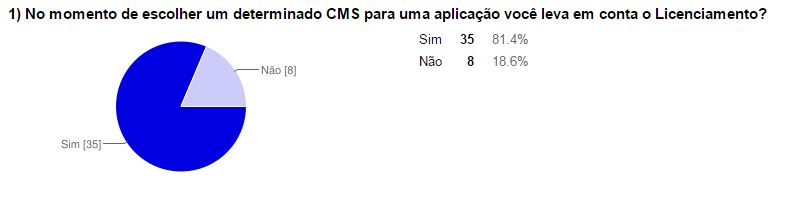
\includegraphics[keepaspectratio=true,scale=0.8]{figuras/Ques_1/q1.jpg}
\caption{Resultado da Questão 1 para o Questionário 1}
\label{Q1_Q1}
\end{figure}

A figura \ref{Q1_Q1} mostra os resultados para questão 1 do questionário que pergunta sobre o licenciamento de software. Nesta questão 81,4\% dos 43 participantes dizem se preocupar com o licenciamento na hora de escolher um determinado CMS, por ter tido uma aceitação muito grande (superior a 75 \%) essa foi uma característica considerada importante.

\begin{figure}[h]
\centering
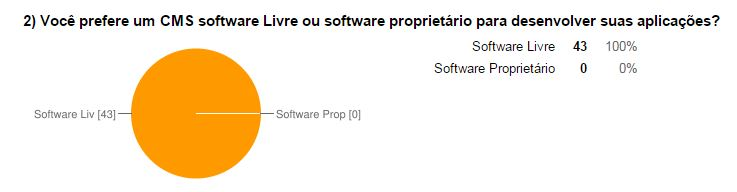
\includegraphics[keepaspectratio=true,scale=0.8]{figuras/Ques_1/q2.jpg}
\caption{Resultado da Questão 2 para o Questionário 1}
\label{Q2_Q2}
\end{figure}

O resultado para a  Questão 2 expresso na figura \ref{Q2_Q2} foi enviesado, pelo fato de que o questionário foi aplicado em comunidades de CMS software livre, e uma comunidade de desenvolvimento web, logo já se esperava que o resultado fosse 100 \% software livre. Se o questionário tivesse sido aplicado em uma determinada empresa que usa CMS proprietário o resultado seria diferente. Porém os 43 entrevistados justificaram a escolha dos CMSs software livre com algumas justificativas levantadas na subquestão 2.1. Essas justificativas em resumo foram:
\begin{itemize}
\item Custos com licença
\item Apoio da comunidade que ajuda de forma colaborativa com o crescimento do CMS
\item Liberdade para customizar o CMS
\item Experiência
\end{itemize}

Um \textit{feedback} de um dos entrevistados foi \textit{"Criar um bom CMS do zero leva tempo e custa muito dinheiro, sendo que existem soluções maduras, prontas para usar, e altamente testadas no mundo do Software Livre"} que justifica os itens a cima.


\begin{figure}[!h]
\centering
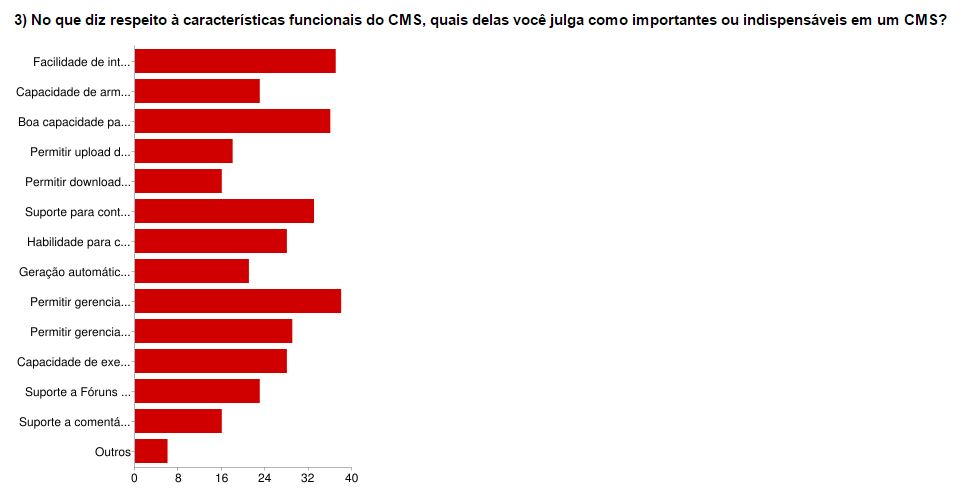
\includegraphics[keepaspectratio=true,scale=0.55]{figuras/Ques_1/q3.jpg}
\caption{Resultado da Questão 3 para o Questionário 1}
\label{Q3_Q3_1}
\end{figure}

\begin{figure}[h]
\centering
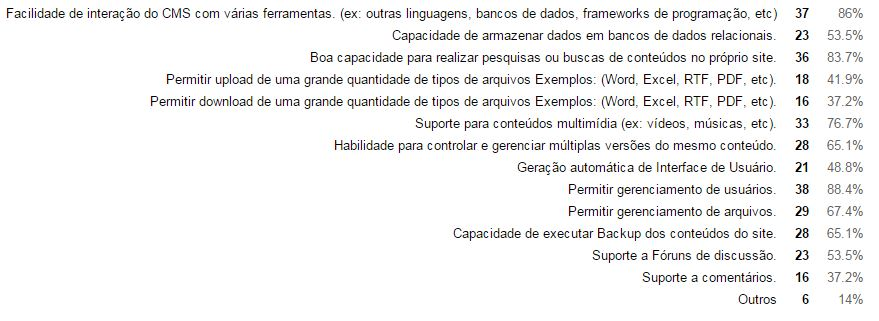
\includegraphics[keepaspectratio=true,scale=0.7]{figuras/Ques_1/q3_1.jpg}
\caption{Resultado da Questão 3 por percentual para o Questionário 1.}
\label{Q3_Q3}
\end{figure}



As figuras \ref{Q3_Q3_1} e \ref{Q3_Q3} estão relacionadas a característica de Adequação Funcional da SQuaRE. Para esta pergunta foram selecionadas 15 características, a fim de perguntar ao entrevistado qual ou quais características são mais importantes em um CMS. Destacaram-se como melhores resultados para essa pergunta:  

    \begin{itemize}
    \item Facilidade que o CMS possui para interagir com várias ferramentas
    \item Capacidade para realizar buscas no próprio site
    \item Suporte para conteúdos multimídias
    \item Permitir o gerenciamento de usuários
    
    \end{itemize}

Para a Questão 3, foram considerados resultados satisfatórios, as características que obtiveram mais de 75 \% de aderência. Além desses resultados no campo outros destacou-se as seguintes respostas: 
% \textcolor{red}{Rever os conceitos de Webservices para baixo}
 \begin{itemize}

   \item Suporte para e-commerce
    \item Extensibilidade
    
    \end{itemize}
    
%\textcolor{red}{Colocar no final}    

%\clearpage


\begin{figure}[!tbh]
\centering
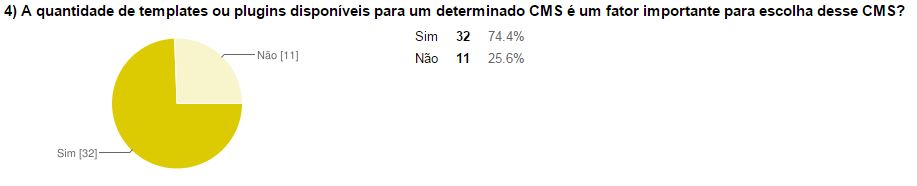
\includegraphics[keepaspectratio=true,scale=0.75]{figuras/Ques_1/q4.jpg}
\caption{Resultado da Questão 4 para o Questionário 1 }
\label{Q4_Q4}
\end{figure}

Para a Questão 4, conforme mostra a Figura \ref{Q4_Q4}, na opnião dos entrevistados, a quantidade de \textit{templates} e \textit{plugins} é importante para escolha de produtos CMS. 


\begin{figure}[!th]
\centering
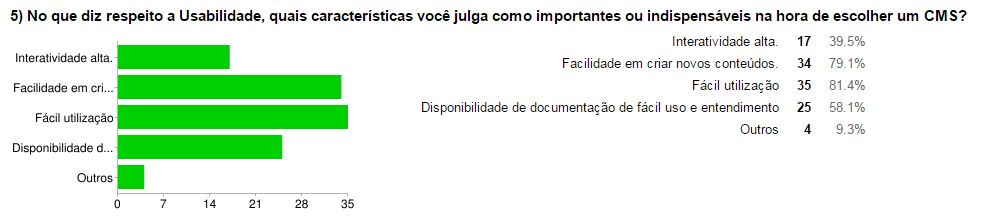
\includegraphics[keepaspectratio=true,scale=0.6]{figuras/Ques_1/q5.jpg}
\caption{Resultado da Questão 5 para o Questionário 1 }
\label{Q5_Q5}
\end{figure}

Na Questão 5, conforme mostra a Figura \ref{Q5_Q5} foi perguntado aos entrevistados sobre a característica de Usabilidade. Nesse quesito destacou-se:

 \begin{itemize}
    \item Fácil Utilização
    \item Facilidade em criar novos conteúdos
    \item Disponibilidade de documentação de fácil uso e entendimento
        
    \end{itemize}

Nesta pergunta, foram considerados os itens que obtiveram mais de 50 \% de aceitação, além disso no campo outros. Os entrevistados sugeriram:
%\textcolor{red}{Rever os 3  primeiros conceitos}
\begin{itemize}
    \item Editor \textit{wysiwyg}\footnote{wysiwyg = What you see is what you get.} robusto.
    \item Padronização da Interface e do Código
    \item Curva de aprendizado
        
    \end{itemize}
    
% \textcolor{red}{Colocar no final}
%Logo, para a construção do método será levado em consideração as características mais bem pontuadas e as características propostas.

\begin{figure}[h]
\centering
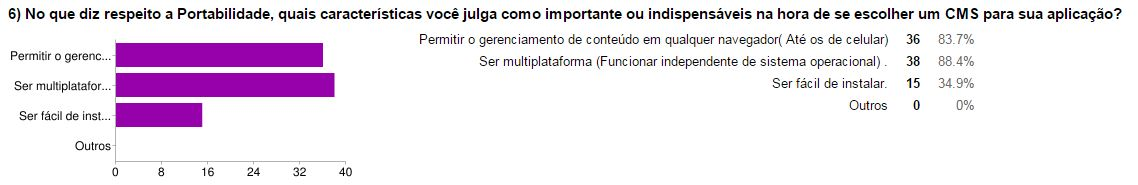
\includegraphics[keepaspectratio=true,scale=0.55]{figuras/Ques_1/q6.jpg}
\caption{Resultado da Questão 6 para o Questionário 1 }
\label{Q6_Q6}
\end{figure}

A Figura \ref{Q6_Q6} mostra os resultados para a característica de Portabilidade. Dois resultados se destacaram com mais de 50 \% foram eles:

\begin{itemize}
    \item Permitir o gerenciamento de conteúdo de qualquer navegador
    \item Ser multiplataforma        
    \end{itemize}

\begin{figure}[h]
\centering
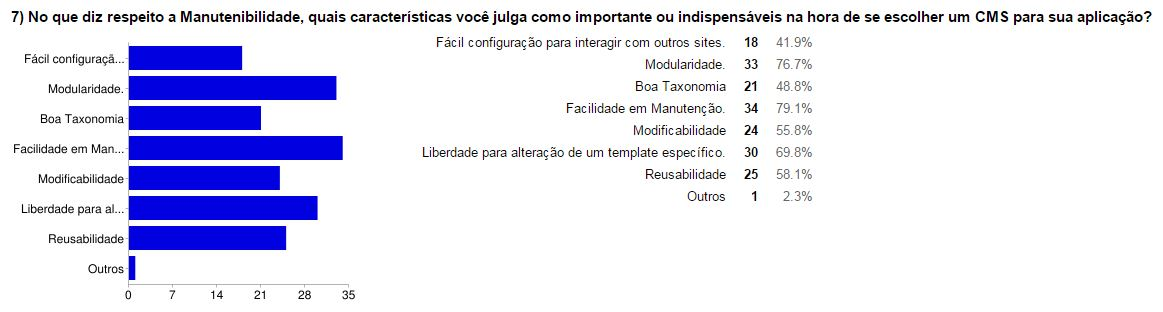
\includegraphics[keepaspectratio=true,scale=0.55]{figuras/Ques_1/q7.jpg}
\caption{Resultado da Questão 7 para o Questionário 1}
\label{Q7_Q7}
\end{figure}

A Questão 7 aborda a característica de Manutenibilidade. De acordo com a Figura \ref{Q7_Q7}, cinco itens se destacaram com mais de 50 \% de aderência. Esses itens foram:

\begin{itemize}
    \item Modularidade
    \item Facilidade em Manutenção
    \item Modificabilidade
    \item Liberdade para alteração de um template específico
    \item Reusabilidade
        
    \end{itemize}
\clearpage    

Um entrevistado disse no campo "outros" que é importante um CMS possuir um  \textit{Framework} de testes.     
    
    
\begin{figure}[!ht]
\centering
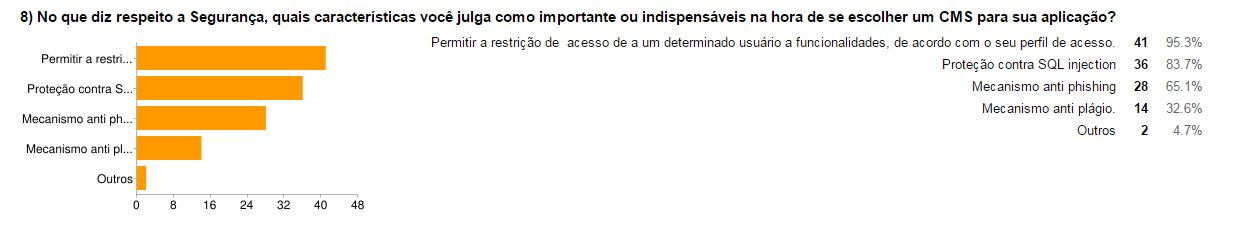
\includegraphics[keepaspectratio=true,scale=0.55]{figuras/Ques_1/q8.jpg}
\caption{Resultado da Questão 8 para o Questionário 1}
\label{Q8_Q8}
\end{figure}

A Figura \ref{Q8_Q8} aborda a característica de Segurança da SQuaRE. Três itens se destacaram com mais de 50 \%. Foram eles:
 

\begin{itemize}
    \item Permitir a restrição de acesso de um determinado usuário
    \item Proteção contra \textit{SQL Injection}
    \item Mecanismo anti \textit{phishing}     
    \end{itemize}
    
Também foi dito no campo "outros" a característica:
"Segurança do código fonte".     
     

\begin{figure}[h]
\centering
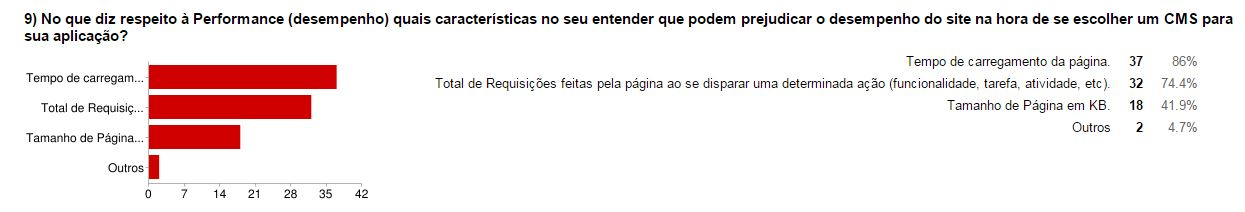
\includegraphics[keepaspectratio=true,scale=0.45]{figuras/Ques_1/q9.jpg}
\caption{Resultado da Questão 9 para o Questionário 1}
\label{Q9_Q9}
\end{figure}

De acordo com a Figura \ref{Q9_Q9}, no que diz respeito ao Desempenho, duas características se destacaram com mais de 50 \% de aderência. Essas características foram:

\begin{itemize}
    \item Tempo de carregamento da página
    \item Total de requisições     
    \end{itemize}
    
No campo outros foi sugerido:


\begin{itemize}
    \item  Quantidade de relacionamentos entre os conteúdos
    \item Configuração de Cache;    
    \end{itemize}
    
\begin{figure}[!htb]
\centering
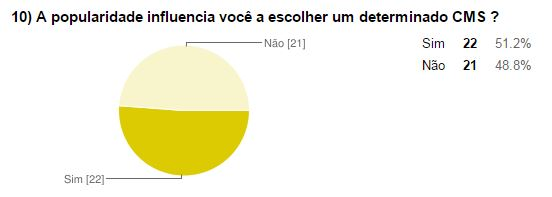
\includegraphics[keepaspectratio=true,scale=0.9]{figuras/Ques_1/q10.jpg}
\caption{Resultado da Questão 10 para o Questionário 1}
\label{Q10_Q1}
\end{figure}


A Figura \ref{Q10_Q1} mostra o resultado para a característica de popularidade. Dos 43 entrevistados, 22 disseram que "Sim" a popularidade influencia na escolha de um determinado CMS; enquanto 21 entrevistados disseram que não influenciam. É possível ver portanto certo equilíbrio nas opniões dos entrevistados. As justificativas dos entrevistados do porquê a popularidade influencia na escolha de um CMS foram: 

\begin{itemize}
    \item  Maior agilidade para resolver questões e aprimorar o CMS
    \item Quanto mais popular, maior a comunidade e melhor a troca de experiências e o suporte oferecido pelos desenvolvedores  
    \item Maior atração para pessoas ajudarem a contribuir com a evolução do CMS
    \item Quanto mais popular, mais recursos são desenvolvidos
    \item Apesar de popularidade não implicar em qualidade, dependendo do projeto na maioria das vezes a seleção dos CMS's candidatos acontece pela popularidade
    \item Um CMS popular traz mais confiança em relação ao seu uso
    \item CMSs mais populares terão mais plugins disponíveis. Isso não torna o CMS melhor, ou garante a qualidade dos plugins, mas é um grande fator para se escolher qual CMS utilizar. Além disso, a comunidade pode ser maior, facilitando possíveis pedidos de suporte  
      
    \end{itemize}

Já os entrevistados que opinaram de forma negativa quanto a popularidade justificaram com os argumentos a seguir:

\begin{itemize}
\item Desde que o CMS disponha de uma boa documentação e cumpra aquilo a que se propõe a popularidade não será ou (deverá) ser um fator importante
\item Um sistema mais popular chama mais a atenção de hackers
\item A adequação do CMS ao foco do projeto é mais importante do que a popularidade da ferramenta escolhida
\item Alguns CMS populares não oferecem recursos avançados
\item Popular não significa que se tenha boa qualidade
\item A usabilidade é um fator mais relevante que a popularidade
\end{itemize}


\begin{figure}[!th]
\centering
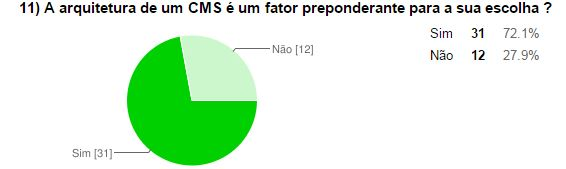
\includegraphics[keepaspectratio=true,scale=0.9]{figuras/Ques_1/q11.jpg}
\caption{Resultado da Questão 11 para o Questionário 1}
\label{Q11_Q1}
\end{figure}


A Figura \ref{Q11_Q1} mostra os resultados da Questão 11 a respeito da arquitetura dos CMSs. 72,1 \% dos entrevistados disseram que sim a arquitetura é um fator que pesa na hora de se escolher um determinado CMS. Em resumo as justificativas dos entrevistados foram as apresentadas a seguir: 

\begin{itemize}
\item Uma boa arquitetura ajuda no entendimento de como o CMS funciona
\item Facilita o uso e aplicação do CMS em questão
\item Define se o site feito com CMS em questão, será extensível ou não
\item Facilita a manutenção 
\item Uma arquitetura extensível e de fácil manutenção é essencial para o desempenho de um CMS robusto. Uma má arquitetura pode inviabilizar o uso do CMS no caso de sites com uma grande quantidade de dados e/ou grande quantidade de page views

\end{itemize}



\begin{figure}[th]
\centering
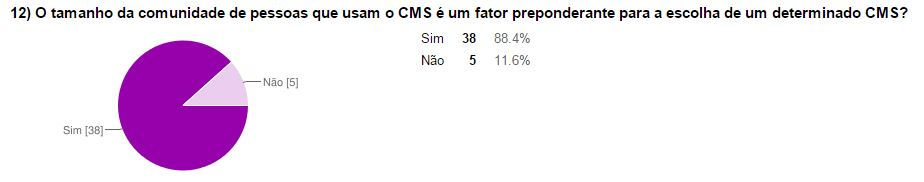
\includegraphics[keepaspectratio=true,scale=0.7]{figuras/Ques_1/q12.jpg}
\caption{Resultado da Questão 12 para o Questionário 1}
\label{Q12_Q1}
\end{figure}
A Figura \ref{Q12_Q1} mostra o resultado para a Questão 12 que diz respeito ao tamanho da comunidade de um determinado CMS. 82 \% dos entrevistados disseram que "Sim" o tamanho da comunidade pesa ao se escolher um determinado CMS. As justificativas para o resultado são apresentadas a seguir:

\begin{itemize}
\item Melhor suporte
\item Muitas pessoas trabalham em prol de objetivos comuns
\item Troca de experiências
\item Melhor índice de confiabilidade, devido à muitos usuários utilizando a mesma plataforma. 
\item Continuidade do projeto

\end{itemize}
\begin{figure}[h]
\centering
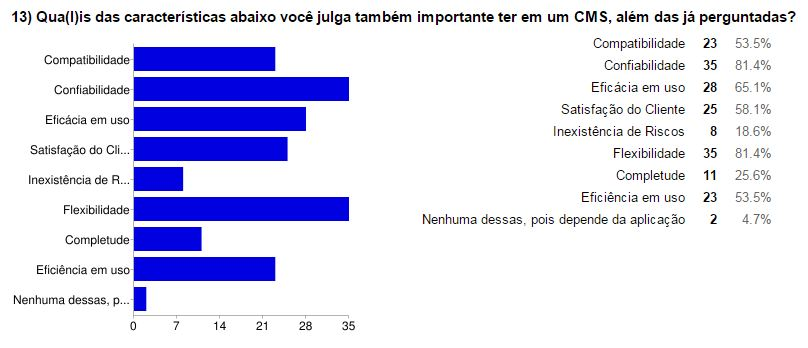
\includegraphics[keepaspectratio=true,scale=0.7]{figuras/Ques_1/q13.jpg}
\caption{Resultado da Questão 13 para o Questionário 1}
\label{Q13_Q1}
\end{figure}

A Figura \ref{Q13_Q1} mostra os resultados para a Questão 13, que pergunta aos entrevistados sobre as características da SQuaRE que não foram mapeadas na literatura. A subcaracterística de Flexibilidade foi inserida nesta questão, pois obteve um grande número de citações na literatura. Foram considerados os resultados com mais de 65 \% de resposta. Esses resultados são apresentados a seguir: 

\begin{itemize}
\item Flexibilidade
\item Confiabilidade
\item Eficácia em Uso

\end{itemize}

Por fim a Questão 14 perguntou aos usuários/especialistas em CMS, se existem mais características importantes e que devem ser levadas em consideração na hora de se escolher um determinado CMS. Em resumo as respostas apresentadas foram:

\begin{itemize}
\item Integração de dados via XML
\item Layouts leves e responsivos
\item Permitir construção de aplicações \textit{mobiles}
\item Extensibilidade
\end{itemize}

%\textcolor{red}{Professor quanto a organização, é melhor que eu divida por seções a análise do questionário? Exemplo: Seção xxxx Resultados questão 1... E assim por diante... }



\section{Visão Geral do Método}
\label{Visao_Método}

O método será composto por duas partes. A primeira parte diz respeito às características que não podem ser mensuradas pela SQuaRE. Já a segunda parte diz respeito às características que podem ser medidas pela SQuaRE. Em ambos os casos serão usadas  as características aprovadas e as características sugeridas pelos especialistas na seção anterior.

A Figura \ref{fig_VisãoMétodo} mostra um fluxograma de execução do método proposto. Os passos vistos na figura serão explicados  nas Seções \ref{M_ParteI} e \ref{M-Parte-II}.

\begin{landscape}
\begin{figure}[h]
\centering
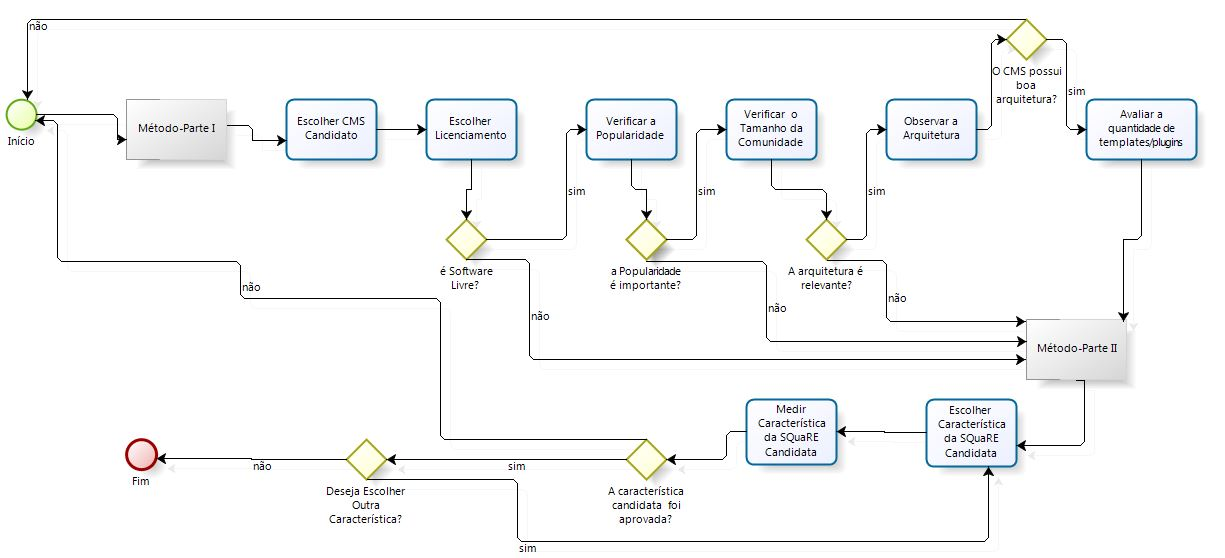
\includegraphics[keepaspectratio=true,scale=0.85]{figuras/MetodoFluxograma.jpg}
\caption{Fluxograma do método proposto }
\label{fig_VisãoMétodo}
\end{figure}

\end{landscape}



\section{Construção do Método - Parte I}

Esta seção tem como objetivo organizar a primeira parte do método que será composta por características que não podem ser mapeadas na SQuaRE.

\subsection{Listagem de características aprovadas pelos especialistas}

Após a aplicação do Questionário 1 (Levantamento de Características de CMS) para os especialistas e a discussão dos resultados, as características que não puderam ser mapeadas pela SQuaRE, mas que foram consideradas importantes foram:

\begin{enumerate}
\item Licenciamento.
\item Popularidade.
\item Tamanho da Comunidade.
\item Arquitetura do CMS.
\item Quantidade de Templates e Plugins disponíveis. 

\end{enumerate}

Estas características foram selecionadas para comporem o método na parte 1. 


\subsection{Passo a passo para a escolha do CMS - Parte I}
\label{M_ParteI}
Esta seção explica como as características listadas no item anterior, relacionam-se para formar uma sequência de passos para o auxílio da escolha de um determinado CMS. O passo a passo apresentado a seguir e corresponde aos passos apresentados na Figura \ref{fig_VisãoMétodo}:

\textbf{Passo 1}: Escolher CMS candidato.
A Seção \ref{free_software} apresenta vários CMSs que podem ser escolhidos, mas existem outras opções que podem também ser usadas, mas que não constam nesta seção.

\textbf{Passo 2}: Verificar qual o Licenciamento do CMS em questão.

No que diz respeito ao Licenciamento está sendo considerado apenas o fato do CMS ser Software Livre ou Software Proprietário. A Seção \ref{free_software} deste trabalho explica as principais diferenças entre os dois tipos de software e apresenta alguns exemplos de CMSs software livre e CMSs software proprietário.

De acordo com os resultados obtidos na Seção \ref{resultados_questionário_1} do \textit{survey} com os  especialistas, a escolha de um CMS software livre é uma boa escolha pelos seguintes motivos:

\begin{itemize}
\item Custos com licença
\item Apoio da comunidade que ajuda de forma colaborativa com o crescimento do CMS
\item Liberdade para customizar o CMS
\item Experiência
\end{itemize}

Porém, caso as preocupações com o custo de licenças sejam irrelevantes, ou não se tenha interesse em nenhum dos fatores citados anteriormente, deve-se prosseguir diretamente para o primeiro passo da segunda parte do método na seção \ref{M-Parte-II}.   

\textbf{Passo 3}: Verificar a popularidade do CMS em questão.

Baseado na escolha de um CMS Software Livre neste passo deve-se analisar a popularidade do CMS em questão.

A Seção \ref{popularidade_CMS} deste trabalho faz uma apresentação dos CMSs mais populares e do porquê a popularidade pode ser importante para um CMS Software Livre. Para os especialistas, a popularidade de um determinado CMS se faz importante pelos motivos apresentados na seção \ref{resultados_questionário_1}. Porém, conforme foi  apontado pelos especialistas na mesma seção, a popularidade pode também não ser um critério relevante na escolha de um determinado CMS. Alguns dos motivos levantados pelos especialistas para que a popularidade não seja levada em consideração:   

\begin{itemize}
\item Desde que o CMS disponha de uma boa documentação e cumpra aquilo a que se propõe a popularidade não será ou (deverá) ser um fator importante.
\item Um sistema mais popular chama mais à atenção de hackers.
\item A adequação do CMS ao foco do projeto é mais importante do que a popularidade da ferramenta escolhida. 
\item A usabilidade é mais relevante que a popularidade.
\end{itemize}

Para se escolher um CMS com base na popularidade podem ser usados um dos três exemplos fornecidos na seção \ref{Cms_vantagens}. 

Caso a popularidade seja considerada importante, deve-se prosseguir para o Passo 4 desta seção, caso contrário siga para o passo 5.

\textbf{Passo 4}: Verificar o Tamanho da Comunidade do CMS em Questão.

A Tabela \ref{Popularidade} e as Figuras \ref{pop_001}, \ref{pop_002}, \ref{pop_003}, \ref{pop_004}, \ref{pop_005} e \ref{pop_006} mostram alguns números para tamanho de comunidade de CMSs levando em consideração redes sociais e o número de \textit{commits} do repositório das aplicações. Além disso, conforme mostra a Figura \ref{Q12_Q1}, mais de 80 \% dos especialistas entrevistados citaram como fatores importantes: 

\begin{itemize}
\item Oferecer um melhor suporte
\item Troca de Experiências
\item Melhor índice de confiabilidade, devido à muitos usuários utilizando a mesma plataforma

\end{itemize} 

Porém caso o tamanho da comunidade não seja importante, deve-se desconsiderar este passo e prosseguir para o passo 5 desta seção.

\textbf{Passo 5}: Observar a arquitetura do CMS em questão.

Neste passo existem dois pontos de decisão chave. O primeiro pergunta ao desenvolvedor se a arquitetura é um fator relevante para a aplicação. Caso seja importante o desenvolvedor deverá investigar a arquitetura do CMS escolhido.

Na Questão \ref{Q11_Q1} os especialistas julgaram que a arquitetura de um CMS se faz importante pelos  motivos apresentados na Seção \ref{resultados_questionário_1}, estes motivos foram:

\begin{itemize}

\item Facilitar o uso e aplicação do CMS em questão
\item Definir se o site feito com o CMS em questão, será extensível ou não
\item Facilitar a manutenção 

\end{itemize}

O segundo ponto chave pergunta se o CMS possui boa arquitetura. Caso tenha o desenvolvedor poderá ir para o próximo passo. Se o CMS não possuir boa arquitetura o desenvolvedor volta para o início do fluxograma, pois uma vez considerada como característica importante pelo desenvolvedor, não sendo aprovada é sinal de que o CMS não será bom para aquele determinado contexto.

Não foram sugeridas métricas para este quesito. Cabe ao desenvolvedor escolher como mensurar e concluir se a arquitetura do CMS em questão é adequada para a sua aplicação.

\textbf{Passo 6}: Avaliar a quantidade de templates e plugins disponíveis no CMS.

Caso este seja um fator relevante para o sucesso da aplicação em questão o próprio responsável por desenvolver a aplicação deve considerar se a quantidade de templates e plugins é relevante para o CMS escolhido.

\section{Construção do Método - Parte II}
\label{M-Parte-II}

Nesta parte do método o objetivo será mapear as características que podem ser medidas com o auxílio das normas SQuaRE. Para esta etapa foi realizado um GQM para identificar e sugerir métricas
para as características estabelecidas como relevantes.   
%Neste capítuleração na hora o será iniciada te a construção desultados so famework0 %. Por necessitar de uma reflexão mais profunda a respeito dos seus objetivos de medições e questões associadas optou-se pelo uso do método GQM (\textit{Goal Question Metric}).


\subsection{Listagem de características aprovadas pelos especialistas}

A Tabela \ref{mapeamento_CMS_características_aprovadas} apresenta  as características relacionadas a qualidade do produto que foram aprovadas pelos especialistas de acordo com a Seção \ref{resultados_questionário_1}. 
As notas de rodapé que explicam as subcaracterísticas mapeadas são referenciadas de acordo com a \citeonline{iso_25023}.

A tabela \ref{mapeamento_CMS_características_aprovadas} foi baseada na Tabela \ref{Cruzamento_Apendice} do Apêndice \ref{Levantamento de características-apendice}, no qual características de CMSs foram relacionadas com suas respectivas características SQuaRE, a fim de identificar quais características necessitam serem medidas.
%\textcolor{red}{Explicar subcaracterísticas que apareceram em notas de rodapé.}
 
	\begin{longtable}{|p{140pt}|p{140pt}|p{120pt}|}
	
	\caption{Cruzamento de Características aprovadas pelos especialistas com características SquaRE - Qualidade do Produto.}
	\label{mapeamento_CMS_características_aprovadas}\\
%  	\end{longtable}

 	\hline
 	 {\raggedright \textbf{Características de CMS aprovadas}}
 	 & {\raggedright \textbf{Características Square}}
 	 & {\raggedright \textbf{Subcaracterísticas Square}}\\
 	\hline
 	 {\raggedright Facilidade que o CMS possui para interagir com várias ferramentas}
 	 & {\raggedright Adequação Funcional}
 	 & {\raggedright Completude Funcional \footnote{Subcaracterística que estabelece que um conjunto de funcionalidades deve abranger todas as tarefas e objetivos específicos dos seus usuários.}}\\
 	\hline
 	 {\raggedright Capacidade para realizar buscas no próprio site.}
 	 & {\raggedright Adequação Funcional}
 	 & {\raggedright Completude Funcional}\\
 	\hline
 	 {\raggedright Suporte para conteúdos multímidia} 
 	 & {\raggedright Adequação Funcional}
& {\raggedright Completude Funcional}\\
 	\hline
{\raggedright Integração de dados via XML}
 	 & {\raggedright Adequação Funcional}
 	 & {\raggedright Completude Funcional}\\
 	\hline
 	 {\raggedright Permitir construção de aplicações \textit{mobiles}}
 	 & {\raggedright Adequação Funcional}
 	 & {\raggedright Completude Funcional}\\
 	\hline
{\raggedright Permitir o gerenciamento de usuários}
 	 & {\raggedright Adequação Funcional}
 	 & {\raggedright Completude Funcional}\\
 	\hline
 	 {\raggedright Suporte para e-commerce}
 	 & {\raggedright Adequação Funcional}
 	 & {\raggedright Completude Funcional}\\
 	\hline
{\raggedright Extensibilidade}
 	 & {\raggedright Adequação Funcional}
 	 & {\raggedright Completude Funcional}\\
 	\hline
{\raggedright Editor wisiwig robusto}
 	 & {\raggedright Adequação Funcional}
 	 & {\raggedright Completude Funcional}\\
 	\hline
 	 {\raggedright Fácil Utilização}
 	 & {\raggedright Usabilidade}
 	 & {\raggedright Operacionalidade \footnote{Subcaracterística que estabelece que um determinado produto ou sistema possui atributos que o tornam fácil de operar e controlar.}}\\
 	\hline
{\raggedright Disponibilidade de documentação de fácil uso e entendimento}
 	 & {\raggedright Usabilidade}
 	 & {\raggedright Aprendizado \footnote{Subcaracterística que estabelece que um produto ou sistema pode ser usado por usuários específicos para atingir metas de aprendizado ao se utilizar um produto com efetividade, eficiência, inexistência de riscos e satisfação em um determinado contexto de uso.} }\\
 	\hline
 	 {\raggedright Facilidade em criar novos conteúdos}
 	 & {\raggedright Usabilidade}
 	 & {\raggedright Operacionalidade}\\\hline

{\raggedright Curva de Aprendizado}
 	 & {\raggedright Usabilidade}
 	 & {\raggedright Aprendizado}\\
 	\hline
 	{\raggedright Layouts Leves e Responsivos}
 	 	 & {\raggedright Usabilidade}
 	 	 & {\raggedright Estética \footnote{Subcaracterística que estabelece que a interface de usuário deve permitir uma interação agradável e satisfatória para o usuário.}}\\
 	 	\hline
 	 {\raggedright Permitir o gerenciamento de conteúdo de qualquer navegador}
 	 & {\raggedright Portabilidade}
 	 & {\raggedright Adaptabilidade \footnote{Subcaracterística que estabelece que um produto ou sistema pode ser adaptado de forma eficaz e eficiente para um hardware, software, ou outros ambientes operacionais de uso.}}\\
 	\hline 
 	{\raggedright Ser multiplataforma}
 	 	 & {\raggedright Portabilidade}
 	 	 & {\raggedright Adaptabilidade}\\
 	 	\hline

 	{\raggedright Modularidade}
 	 	 	 & {\raggedright Manutenibilidade}
 	 	 	 & {\raggedright Modularidade \footnote{Subcaracterística que estabelece que um software, ou sistema possui componentes discretos, tais que a mudança para um componente tem um impacto mínimo sobre outros componentes.}}\\
 	 	 	\hline
	{\raggedright Modificabilidade}
 	 	 	 & {\raggedright Manutenibilidade}
 	 	 	 & {\raggedright Modificabilidade\footnote{Subcaracterística que estabelece que um produto ou sistema pode ser modificado de forma eficaz e eficiente sem introduzir defeitos.}}\\
 	 	 	\hline
	{\raggedright Liberdade para alteração de um template específico}
 	 	 	 & {\raggedright Manutenibilidade}
 	 	 	 & {\raggedright Modificabilidade}\\
 	 	 	\hline
	{\raggedright Reusabilidade}
 	 	 	 & {\raggedright Manutenibilidade}
 	 	 	 & {\raggedright Reusabilidade \footnote{Subcaracterística que estabelece que um componente pode ser utilizado em mais do que um sistema, ou na construção de outros ativos.}}\\
 	 	 	\hline
	{\raggedright Padronização da interface e do código}
 	 	 	 & {\raggedright Manutenibilidade}
 	 	 	 & {\raggedright Reusabilidade}\\
 	 	 	\hline
	{\raggedright \textit{Framework} de testes}
 	 	 	 & {\raggedright Manutenibilidade}
 	 	 	 & {\raggedright Testabilidade \footnote{ Subcaracterística que estabelece a possibilidade de determinar critérios de teste para um dado produto, sistema, ou componente.}}\\
 	 	 	\hline
{\raggedright Permitir a restrição de acesso de um determinado usuário}
 	 & {\raggedright Segurança}
 	 & {\raggedright Confidencialidade \footnote{ Subcaracterística que estabelece que um produto ou sistema garante que os dados são acessíveis somente por pessoas autorizadas ao acesso.}}\\
 	\hline
 	 {\raggedright Proteção contra \textit{SQL Injection}}
 	 & {\raggedright Segurança}
 	 & {\raggedright Integridade \footnote{Subcaracterística que estabelece que um sistema, produto ou componente deve impedir o acesso não autorizado ou a modificação de dados.}}\\
 	\hline
 {\raggedright Mecanismo anti \textit{phishing}}
 	 & {\raggedright Segurança}
 	 & {\raggedright Integridade}\\
 	\hline
 	 {\raggedright Segurança do código fonte}
 	 & {\raggedright Segurança}
 	 & {\raggedright Integridade}\\\hline

{\raggedright Tempo de carregamento da página}
 	 & {\raggedright Eficiência de Desempenho}
 	 & {\raggedright Comportamento do Tempo \footnote{Subcaracterística que estabelece que os tempos de resposta, de processamento e as taxas de transferência de um produto ou sistema devem atender aos requisitos.}}\\
 	\hline
 	 {\raggedright Total de requisições}
 	 & {\raggedright Eficiência de Desempenho}
 	 & {\raggedright Utilização de Recursos}\\
 	\hline 
 	{\raggedright Quantidade de relacionamentos entre os conteúdos}
 	 	 & {\raggedright Eficiência de Desempenho}
 	 	 & {\raggedright Utilização de Recursos \footnote{Subcaracterística que estabelece que as quantidades de recursos utilizados por um produto, ou sistema devem atender aos requisitos.}}\\
 	 	\hline
{\raggedright Configuração de Cache}
 	 & {\raggedright Eficiência de Desempenho}
 	 & {\raggedright Utilização de Recursos}\\
 	\hline
 	 		{\raggedright Confiabilidade}
 	 	 	 	 	 & {\raggedright Confiabilidade}
 	 	 	 	 	 & {\raggedright Maturidade\footnote{Subcaracterística que estabelece que um sistema deve satisfazer as necessidades de confiabilidade en operação normal.},
 	 	 	 	 	 Tolerância a Falhas \footnote{Subcaracterística que estabelece que um sistema, produto ou componente deve operar como pretendido, apesar da presença de falhas de hardware ou software.}
 	 	 	 	 	 Capacidade de Recuperação\footnote{Subcaracterística que estabelece que em caso de uma interrupção ou falha, um produto ou sistema pode recuperar os dados diretamente afetados e restabelecer o estado desejado do sistema.} e
 	 	 	 	 	 Disponibilidade\footnote{Subcaracterística que estabelece que um sistema, produto, ou componente está operacional e acessível quando necessário para uso.} 
 	 	 	 	 	 }\\
 	 	 	 	 	\hline	
 	\end{longtable}
De forma semelhante a Tabela \ref{mapeamento_CMS_características_aprovadas_qualidade_em_uso} apresenta as características de qualidade em uso aprovadas pelos especialistas.

\begin{longtable}{|p{140pt}|p{140pt}|p{120pt}|}
	
	\caption{Cruzamento de Características aprovadas pelos especialistas com características SquaRE - Qualidade em uso.}
	\label{mapeamento_CMS_características_aprovadas_qualidade_em_uso}\\
%  	\end{longtable}

 	\hline
 	 {\raggedright \textbf{Características de CMS aprovadas}}
 	 & {\raggedright \textbf{Características Square}}
 	 & {\raggedright \textbf{Subcaracterísticas Square}}\\
 	\hline
 	 {\raggedright Flexibilidade}
 	 & {\raggedright Cobertura de Contexto}
 	 & {\raggedright Flexibilidade\footnote{Subcaracterística que estabelece o quanto um produto ou sistema pode ser utilizado de forma eficaz, de forma eficiente, livre de riscos e com satisfação em contextos além daqueles definidos inicialmente na especificação de requisitos. \cite{iso_25022} }}\\
 	\hline
 	 {\raggedright Efetividade}
 	 & {\raggedright Efetividade}
 	 & {\raggedright Efetividade}\\
 	\hline
 
\end{longtable}

\subsection{Passo a passo para a escolha do CMS - Parte II}
\label{passo_parteII_metodo}

\textbf{Passo 1}: Escolher Característica(s) SQuaRE candidata(s).

O objetivo deste passo é escolher entre uma, ou várias das características listadas abaixo para serem medidas no passo 2.

De acordo com as tabelas \ref{mapeamento_CMS_características_aprovadas} e \ref{mapeamento_CMS_características_aprovadas_qualidade_em_uso} as características SQuaRE que apareceram foram:

\begin{itemize}
%\renewcommand{\labelitemi}{-}
\item Adequação Funcional
\item Usabilidade
\item Manutenibilidade
\item Portabilidade
\item Segurança
\item Eficiência de Desempenho 
\item Confiabilidade
\item Eficácia em Uso ou Efetividade
\item Cobertura de Contexto
\end{itemize}

Neste passo, antes de escolher uma destas características, observe os seguintes questionamentos que podem ser usados na escolha das características que podem ser analisadas:

\begin{enumerate}
\item Para a aplicação em questão é importante o CMS cumprir com suas funcionalidades? Exemplo: O CMS deve possuir boa capacidade para realizar buscas?; O CMS deve ser extensível? etc. 

\item Para a aplicação em questão é importante o CMS ter um bom consumo de recursos de hardware, como memória e recursos de entrada e saída?

\item Para a aplicação em questão é importante que o usuário tenha facilidade para desenvolver sua aplicação com CMS?

\item Para a aplicação em questão é importante que o CMS possua uma curva de aprendizado baixa?

\item Para a aplicação em questão é importante que o CMS tenha documentação disponível?

\item Para a aplicação em questão é importante o CMS proteger os dados do usuário e prover um certo nível de restrição de acesso?

\item Para a aplicação em questão é importante CMS possa ser modificado ou mantido por desenvolvedores?

\item Para a aplicação em questão é importante o CMS se adequar a vários browsers diferentes?

\item Para a aplicação em questão é importante que o CMS possua flexibilidade no seu contexto de uso?

\item Para a aplicação em questão é importante que os usuários consigam realizar suas tarefas de forma completa atingindo todos os seus objetivos?

\end{enumerate}

%Caso sejam importantes para a aplicação os questionamentos:

Para saber qual questionamento cada pergunta se refere utilize a Tabela \ref{Decisao}. Escolha as características com base nos questionamentos que são mais relevantes para a sua aplicação.
%
%\begin{itemize}
%\item 1 - A característica que deve ser escolhida para ser medida é a de \textit{Adequação Funcional}.
%\item 2 - A característica que deve ser escolhida para ser medida é a de \textit{Eficiência de Desempenho}.
%\item 3, 4, ou 5 - A característica que deve ser escolhida para ser medida é a de \textit{Usabilidade}.
%\item 6 - A característica que deve ser escolhida para ser medida é a de \textit{Segurança}.
%\item 7 - A característica que deve ser escolhida para ser medida é a de \textit{Manutenabilidade}.
%\item 8 - A característica que deve ser escolhida para ser medida é a de \textit{Portabilidade}.
%\item 9 - A característica que deve ser escolhida para ser medida é a de \textit{Cobertura do Contexto}. 
%\item 10 - A característica que deve ser escolhida para ser medida é a de \textit{Eficácia em Uso}. 
%\end{itemize}


\begin{longtable}{|p{95pt}|p{150pt}|}
 	\caption{Tomada de decisão} 
 	\label{Decisao}\\
 	\hline
 	{\raggedright \textbf{Questionamento}}
 	 	 	 & {\raggedright {\textbf{Característica}}}\\
 	 	\hline
 	 {\raggedright \textbf{1}}
 	 & {\raggedright {\textit{Adequação Funcional}}}\\	
 	\hline
 		{\raggedright \textbf{2}}
 	 	 & {\raggedright \textit{Eficiência de Desempenho}}\\	 	
 	 	\hline
 	 {\raggedright \textbf{3}}
 	 & {\raggedright  \textit{Usabilidade} }\\
 	
 	\hline
 	 {\raggedright \textbf{4}}
 	 & {\raggedright \textit{Usabilidade}} 	
 \\	\hline
 	 {\raggedright \textbf{5}} 
 	 & {\raggedright  \textit{Usabilidade}} \\
	\hline
 	 {\raggedright \textbf{6}}
 	 & {\raggedright \textit{Segurança}} 
 	\\\hline
 	{\raggedright \textbf{7}}
 	 & {\raggedright \textit{Manutenabilidade}}
  	                \\\hline
 	{\raggedright \textbf{8}}
 	 & {\raggedright \textit{Portabilidade}}
 	  \\
 
 	\hline
 	{\raggedright \textbf{9}}
 	 	 & {\raggedright \textit{Cobertura de Contexto}}
 	 	  \\
 	 
 	 	\hline
 	{\raggedright \textbf{10}}
 	 	 & {\raggedright \textit{Efetividade}}
 	 	  \\
 	 
 	 	\hline
 	 
\end{longtable}

\textbf{Passo 2}: Medir Característica da SQuaRE candidata.

Baseado nas escolhas do passo 1 desta seção as características escolhidas devem ser submetidas as medições encontradas no apêndice \ref{GQM-Métricas-Apendice}. 
Após a execução das métricas deve-se observar os resultados para seguir o fluxograma proposto na imagem \ref{Visao_Método}. Caso o resultado da medição associada não seja satisfatório, deve-se voltar ao passo inicial do método na seção \ref{M_ParteI}.
%\textbf{Passo 2}: Definir um número final  para as Característica de \textit{Usabilidade} de acordo com as métricas deerísticfinidas na seção \ref{Questões-Métricas}.
%
%\textbf{Passo 3}: Definir um número final  para as Característica de \textit{Portabilidade} de acordo com as métricas definidas na seção \ref{Questões-Métricas}.
%
%\textbf{Passo 4}: Definir um número final  para as Característica de \textit{Manutenabilidade} de acordo com as métricas definidas na seção \ref{Questões-Métricas}.
%
%\textbf{Passo 5}: Definir um número final  para as Característica de \textit{Segurança} de acordo com as métricas definidas na seção \ref{Questões-Métricas}.
%
%\textbf{Passo 6}: Definir um número final  para as Característica de \textit{Eficiência de Desempenho} de acordo com as métricas definidas na seção \ref{Questões-Métricas}.
%
%\textbf{Passo 7}: Definir um número final  para as Característica de \textit{Confiabilidade} de acordo com as métricas definidas na seção \ref{Questões-Métricas}.
%
%\textbf{Passo 8}: Definir um número final  para a  Característica de \textit{Cobertura de contexto} de acordo com as métricas definidas na seção \ref{Questões-Métricas}.
%
%\textbf{Passo 9}: Definir um número final  para a  Característica de \textit{Cobertura de contexto} de acordo com as métricas definidas na seção \ref{Questões-Métricas}.
%
%A definição da fórmula para o número final será apresentada na seção \ref{Número-Final}

\subsection{Objetivo de Medição}

Para delimitar o objetivo de medição foram usados os templates definidos nas Tabelas \ref{ObjMed} e \ref{ObjMed-2}:

\begin{longtable}{|p{160pt}|p{265pt}|}
 	\caption{Objetivo de Medição \cite{sollingen}.} \label{ObjMed}\\
 	\hline
 	 {\raggedright \textbf{Analisar}}
 	 & {\raggedright {O CMS em estudo}}\\
 	
 	\hline
 	 {\raggedright \textbf{Para o propósito de}}
 	 & {\raggedright   Conhecer }\\
 	
 	\hline
 	 {\raggedright \textbf{Com respeito a}}
 	 & {\raggedright Qualidade do Produto segundo a SQuaRE (ISO/IEC 25010,2011)}\\
 	
 	\hline
 	 {\raggedright \textbf{Do ponto de vista}} 
 	 & {\raggedright Do pesquisador 	                 } \\

 	\hline
 	 {\raggedright \textbf{No contexto}}
 	 & {\raggedright De aplicação do CMS em funcionamento num determinado site.} \\
 	\hline
\end{longtable}

\begin{longtable}{|p{160pt}|p{265pt}|}
 	\caption{Objetivo de Medição \cite{sollingen}.} \label{ObjMed-2}\\
 	\hline
 	 {\raggedright \textbf{Analisar}}
 	 & {\raggedright {O CMS em estudo}}\\
 	
 	\hline
 	 {\raggedright \textbf{Para o propósito de}}
 	 & {\raggedright   Conhecer }\\
 	
 	\hline
 	 {\raggedright \textbf{Com respeito a}}
 	 & {\raggedright Qualidade em Uso segundo a SQuaRE (ISO/IEC 25010,2011)}\\
 	
 	\hline
 	 {\raggedright \textbf{Do ponto de vista}} 
 	 & {\raggedright Do pesquisador 	                 } \\

 	\hline
 	 {\raggedright \textbf{No contexto}}
 	 & {\raggedright De aplicação do CMS em funcionamento num determinado site.} \\
 	\hline
\end{longtable}

\subsection{Questões}
\label{Questões-GQM}
As questões definidas de acordo com o objetivo de medição foram:

\begin{enumerate}

\item Qual o percentual ( \%) de completude funcional existente em um determinado CMS?
\item O usuário consegue realizar tarefas no CMS com sucesso?
\item O CMS em questão possui curva de aprendizada baixa?
\item A estética (layout) do CMS é proporciona uma boa experiência para o usuário?
\item O CMS consegue se adaptar a diversos browser, ou sistemas operacionais?
\item Como os componentes que pertencem a um determinado módulo do CMS se relacionam?
\item Os módulos do CMS são reusáveis?
\item O usuário pode modificar um determinado template ou plugin conforme a sua necessidade?
\item O CMS possui algum nível de teste? Exemplos: unidade, aceitação, sistema, integração, regressão.
\item O CMS permite controlar o acesso de seus usuários?
\item O CMS possui proteção contra ataques web? Exemplos: SQL Injection, RFI, Cookie Poisoning?
\item Quanto tempo o CMS leva para carregar uma determinada página?
\item A quantidade de relacionamentos entre os módulos do CMS afeta o desempenho deste CMS?
\item O CMS oferece confiablidade quando usado?
\item O CMS possui flexibilidade em uso?
\item O CMS é eficaz no seu uso?




\end{enumerate}

\subsection{Métricas}
\label{GQM-Métricas}

As métricas definidas de acordo com as questões estão mapeadas no Apêndice \ref{GQM-Métricas-Apendice}. As métricas estão agrupadas por seções que descrevem as características da SQuaRE mapeadas.  

As figuras \ref{GQM-Diagrama_1} e \ref{GQM-Diagrama_2} apresentam o mapeamento dos objetivos de medição, suas questões e respectivas métricas associadas.

\begin{figure}[h]
\centering
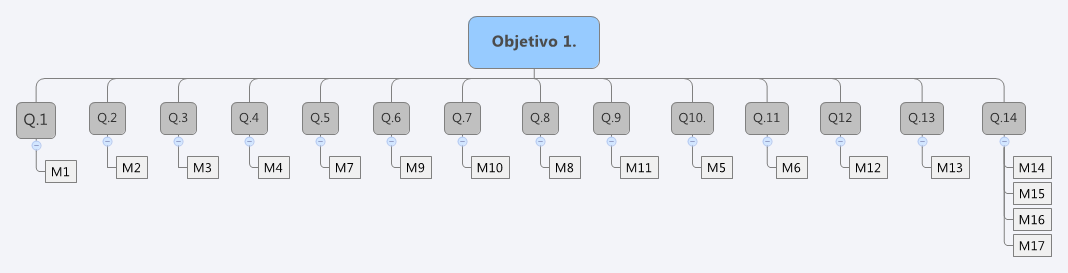
\includegraphics[keepaspectratio=true,scale=0.45]{figuras/GQM-Diagrama1.png}
\caption{Diagrama GQM para a Qualidade do Produto}
\label{GQM-Diagrama_1}
\end{figure}



\begin{figure}[h]
\centering
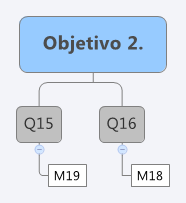
\includegraphics[keepaspectratio=true,scale=0.8]{figuras/GQM-Diagrama2.png}
\caption{Diagrama GQM para Qualidade em Uso }
\label{GQM-Diagrama_2}
\end{figure}

\clearpage
\section{Análise de resultados para o segundo questionário}
\label{resultados_quest2}

Para a validação das métricas elaboradas foi construído um novo questionário. Este questionário está descrito na Seção \ref{Questionário_2} do Apêndice \ref{Questionários}. Os procedimentos de aplicação do questionário e o detalhamento da sua estrutura estão presentes nas Seções \ref{Instrumentos_de_coleta} e \ref{procedimentos}. Esta seção tem como objetivo mostrar o processo de validação do segundo questionário.

\subsection{Procedimentos necessários para a execução da Análise de Fatores}

A análise de fatores tem como principal objetivo expressar um grande número de variáveis em uma quantidade pequena de fatores. A análise de fatores observa padrões de correlações. As correlações representam o relacionamento entre as variáveis envolvidas \cite{dancey}. 

Segundo os mesmos autores, grupos de variáveis altamente correlacionadas entre si formam um fator. Um fator consiste em uma variável hipotética, no qual os seus participantes diferem.

\citeonline{dancey} sugerem que para executar a análise de fatores alguns passos devem ser seguidos, estes passos são:

\begin{enumerate}
\item \textbf{Produzir a matriz de correlações.\footnote{A matriz de correlações gerada equivale ao conjunto de respostas fornecidos pelo sujeito. Ela é 80 X 19. Em que 80 é a quantidade de respostas fornecidas pelos sujeitos (linhas da matriz) e 19  o número de questões do \textit{survey}(colunas da matriz).}}

\item \textbf{Extrair um conjunto de fatores:} O objetivo desta etapa é extrair o mínimo de fatores considerando o máximo de variação. Porém, a decisão sobre o número de fatores a serem extraídos cabe ao pesquisador, que se fundamenta tanto em critérios estatísticos quanto teóricos.

\item \textbf{Determinar o número de fatores que deve ser considerado}: uma boa prática para determinar o número de fatores é analisar o gráfico de declividade. O gráfico de declividade relaciona o número de fatores plotados com a quantidade de variância. O gráfico traz a ideia que os fatores decrescem até certo nível e depois se estabilizam formando uma linha horizontal. Como regra observa-se o gráfico e encontra-se o ponto onde o gráfico começa a ficar horizontal. A partir disso, adota-se como fator os pontos demarcados antes ao ponto em que o gráfico começa a se estabilizar. O ponto de estabilização é definido como o ponto com valor próprio igual a 1 (Regra de Kaizer)\cite{maroco2013}.  

\item\textbf{ Verificar as cargas fatoriais}: As cargas fatoriais informam o relacionamento dos itens com os fatores. É uma boa prática encontrar cargas fatoriais de uma matriz rotacionada. O processo de rotação da matriz pode ser por métodos ortogonais (\textit{Varimax, Equamax}), ou por métodos oblíquos (\textit{Direct Oblimin, Promax}) \cite{maroco2013}. 


As rotações ortogonais são mais fáceis de reportar e de interpretar . Porém, o pesquisador deve assumir que os construtos\footnote{Instrumentos de Coleta} são independentes (na prática essa restrição é mais difícil de ser respeitada). Por sua vez, as rotações oblíquas permitem que os fatores sejam correlacionados. Entretanto, são mais difíceis de descrever e interpretar \cite{maroco2013}. 

\item \textbf{Nomear os fatores encontrados}: Após a rotação, o pesquisador deve observar as cargas fatoriais, a fim de encontrar conjuntos de variáveis comuns. Para isso, a decisão  pode ser tomada com base no valor da carga que deve ser incluída. Este processo de escolha do valor da carga base tende a ser arbitrário, porém é de costume escolher uma carga base que varie de 0,3 a 0,5.

\end{enumerate}

\subsection{Resultados obtidos - Validação da matriz de dados}

Antes de iniciar a análise de dados, foi necessária a validação da matriz de dados. Esta validação foi realizada com o auxílio do Software \textit{IBM SPSS Statistics }\circledR \footnote{Disponível em: http://www-03.ibm.com/software/products/pt/spss-statistics}. 

Para a validação da matriz de dados obtida por meio dos resultados fornecidos pelos sujeitos foram usados três índices:

\begin{enumerate}

\item \textbf{ \textit{ $\alpha$ de Cronbach}}: serve para indicar a \textbf{confiabilidade} de um dado construto. O índice $\alpha$ estima  o quão uniforme os itens contribuem para a soma não ponderada do instrumento, variando numa escala de 0 a 1. Esta propriedade é conhecida por consistência interna da escala e, assim, o $\alpha$ pode ser interpretado como coeficiente médio de todos as estimativas de consistência interna que se obteriam se todas as divisões possíveis da escala fossem feitas \apud{Cronbach}{maroco2013}. Para \apudonline{Nunnaly}{maroco2013} , um instrumento possui boa confiabilidade se o $\alpha$ de Cronbach associado é > = 70 \% . 

\item \textbf{\textit{Kaiser-Meyer-Olklin (KMO)}}: serve para indicar a \textbf{consistência dos dados} da matriz em questão. O KMO indica a proporção das variâncias dos dados que podem ser consideradas comuns a todas as variáveis envolvidas. O teste KMO varia entre 0 e 1. Quanto mais perto de 1 melhor, porém para ser aceitável o KMO deve ser >= 0,5 \apud{Hair}{figueiredo2010}. 

\item \textit{\textbf{Esfericidade de Bartlett (BTS)}}: serve para indicar se existem \textbf{correlações não nulas} entre as variáveis presentes na matriz de dados. O BTS verifica a hipótese nula de que a matriz de dados é uma matriz identidade. Caso essa hipótese seja rejeitada, então existe consistência entre os dados e a análise fatorial pode ser aplicada \apud{Ferreira_2004}{carneiro_2009}. O teste BTS para ser aceitável deve ser < = 0,05 \apud{Hair}{figueiredo2010}.  

\end{enumerate}

Após a submissão da matriz de dados no Software SPSS obteve-se como resultados para os indicadores, os dados mostrados na tabela \ref{Resultados_indicadores}:

% Table generated by Excel2LaTeX from sheet 'Plan1'
\begin{table}[htbp]
  \centering
  \caption{Resultados para os indicadores estabelecidos}
    \begin{tabular}{|r|r|r|}
   \hline
          & \textbf{Critério de aceitação} & \textbf{Resultado obtido} \\\hline
   \textbf{ $\alpha$} & > = 0,7 & 0,746 \\\hline
   \textbf{ KMO}   & > = 0,5 & 0,636 \\\hline
   \textbf{ BTS}   & < = 0,05 & 0,000 \\\hline
    \end{tabular}%
  \label{Resultados_indicadores}%
\end{table}%

A partir dos dados apresentados conclui-se que a matriz de dados é válida e que pode ser fatorada, isto é, reduzida em fatores.
 



\subsection{Extração de fatores}
\label{ExtraçãodeFatores}
Para a encontrar a quantidade de fatores existentes na matriz de dados, foi gerado um gráfico de declividade. A Figura \ref{grafico_declividade} mostra o cruzamento dos valores próprios\footnote{Número que representa o quanto um fator é relevante para o conceito. } com o número de questões existentes. 

\begin{figure}[!htb]
\centering
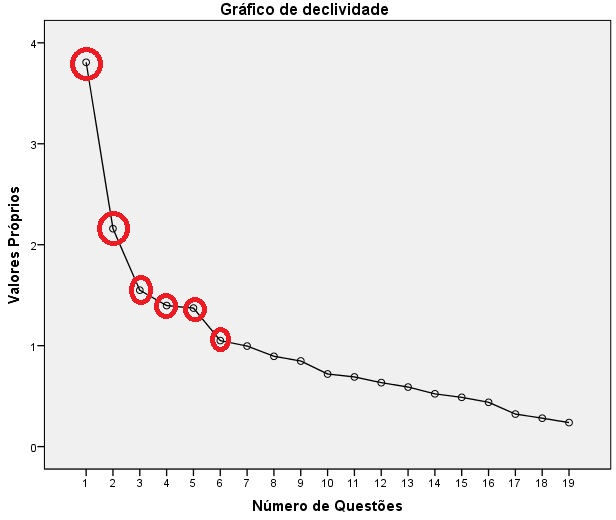
\includegraphics[keepaspectratio=true,scale=0.5]{figuras/Ques_2/graficodeclividade.jpg}
\caption{Gráfico de declividade para a matriz de dados}
\label{grafico_declividade}
\end{figure}

Os pontos circulados mostram as declividades que representam os fatores. Após o par de pontos (7,1), isto é, após a questão 7 ocorre a estabilização do gráfico, onde o valor próprio já está abaixo de 1. O gráfico sugere seis fatores nos quais as questões elaboradas podem ser agrupadas. 

Foi escolhida a rotação oblíqua \textit{Direct Oblimin}, porque de acordo com os autor \cite{DAMASIO2012} ela busca uma solução simples com maior correlação entre os fatores envolvidos.

Quanto ao valor mínimo de aceitação para as cargas de fatores, foi fixado o valor de 0,3; valor semelhante ao usado por \citeonline{maroco2013} e dentro do intervalo sugerido por \citeonline{dancey} em suas pesquisas.




Do ponto de vista teórico o agrupamento de questões para 6 fatores como indicado na Tabela \ref{6-fatores} do Apêndice \ref{cargas_fatoriais_apendice} e da Figura \ref{grafico_declividade}, não apresenta nenhuma semelhança do ponto de vista da literatura SQuaRE. Isto é, tomando como exemplo o Fator 2, que é composto pelos conceitos Confidencialidade, Disponibilidade e Tolerância a Falhas, observa-se que estes conceitos pertencem a características diferentes da SQuaRE (Segurança e Confiabilidade). Estes conceitos não se relacionam. Com esta motivação, foram feitas reduções no número de fatores buscando alguma semelhança com a SQuaRE. Além disso, o gráfico de declividade mostra que os fatores possuem um valor próprio bastante próximo, o que indica que os fatores podem ser reduzidos.


A título de exercício foram citadas outras soluções fatoriais, com cinco, quatro, três e dois fatores. As Tabelas \ref{5-fatores}, \ref{4-fatores}, \ref{3-fatores}, \ref{2-fatores} do Apêndice \ref{cargas_fatoriais_apendice} exemplificam estas reduções. No entanto, a solução fatorial que mais se aproximou da literatura foi a de 1 fator, como mostra a Tabela \ref{1-fator}.
       
     
          \begin{longtable}{rr}
          \caption{Cargas fatoriais para um  fator}
                         \label{1-fator}
          \\\hline
          \multicolumn{2}{c}{\textbf{Matriz de componentes - um fator}} \\
          \hline
          \multicolumn{1}{l}{\multirow{2}[2]{*}{\textbf{Questão - Conceito}}} & \multicolumn{1}{c}{\textbf{Componente}} \\
          \multicolumn{1}{l}{} & \multicolumn{1}{c}{\textbf{1}} \\
          \multicolumn{1}{l}{\textbf{Q1 - Completude Funcional}} & 0,237 \\
          \multicolumn{1}{l}{\textbf{Q2 - Operacionalidade}} & \textbf{0,340} \\
          \multicolumn{1}{l}{\textbf{Q3 - Aprendizado}} & 0,265 \\
          \multicolumn{1}{l}{\textbf{Q4 - Estética}} & \textbf{0,662} \\
          \multicolumn{1}{l}{\textbf{Q5 - Confidencialidade}} & 0,075 \\
          \multicolumn{1}{l}{\textbf{Q6 - Integridade}} & 0,090 \\
          \multicolumn{1}{l}{\textbf{Q7- Adaptabilidade}} & \textbf{0,353} \\
          \multicolumn{1}{l}{\textbf{Q8 - Modificabilidade}} & \textbf{0,389} \\
          \multicolumn{1}{l}{\textbf{Q9 - Reusabilidade}} & \textbf{0,423} \\
          \multicolumn{1}{l}{\textbf{Q10 - Modularidade}} & \textbf{0,539} \\
          \multicolumn{1}{l}{\textbf{Q11 - Testabilidade}} & \textbf{0,640} \\
          \multicolumn{1}{l}{\textbf{Q12 - Comportamento do Tempo}} & \textbf{0,652} \\
          \multicolumn{1}{l}{\textbf{Q13 - Utilização de Recursos}} & \textbf{0,548} \\
          \multicolumn{1}{l}{\textbf{Q14 - Maturidade}} & \textbf{0,476} \\
          \multicolumn{1}{l}{\textbf{Q15 - Disponibilidade}} & 0,279 \\
          \multicolumn{1}{l}{\textbf{Q16 - Tolerância a Falhas}} & \textbf{0,377} \\
          \multicolumn{1}{l}{\textbf{Q17 - Recuperabilidade}} & \textbf{0,702} \\
          \multicolumn{1}{l}{\textbf{Q18 - Efetividade}} & \textbf{0,410} \\
          \multicolumn{1}{l}{\textbf{Q19 - Flexibilidade}} & \textbf{0,355} \\
          \hline
          \end{longtable}%
       
Foi observado que alguns conceitos não possuem carga fatorial suficiente. Considerando o contexto do trabalho elaborado, esta divisão não apresenta restrições quanto a sua organização, logo todos os conceitos presentes no Fator 1 podem ser chamados de \textit{métricas mais significativas} para os especialistas. Conclui-se, então, que as métricas mais significativas para o estudo são as que possuem carga fatorial >= 0,3 no Fator 1. 

Porém, ainda podem ser percebidas algumas métricas menos significantes, isto é possuem carga fatorial abaixo do estabelecido. Observando as métricas excluídas, nota-se que alguns dos conceitos que foram considerados importantes no decorrer do trabalho como a Adequação Funcional (Completude Funcional) e a Segurança (Confidencialidade, Integridade), ficaram de fora do fator por não terem carga fatorial suficiente. 

A partir das métricas com carga fatorial insignificante foi feita a média e o desvio padrão, a fim de estabelecer uma análise mais completa dos dados. A Tabela  \ref{MediaExcluidos} mostra esses dados.



\begin{table}[htbp]
  \centering
  \caption{Média e Desvio Padrão para questões com carga fatorial insuficiente.}
    \begin{tabular}{llrrrrr}
    \toprule
    \multicolumn{2}{l}{} & \multicolumn{1}{c}{Q1} & \multicolumn{1}{c}{Q3} & \multicolumn{1}{c}{Q5} & \multicolumn{1}{c}{Q6} & \multicolumn{1}{c}{Q15} \\
    \midrule
    \multicolumn{2}{l}{Média} & 3,688 & 3,625 & 3,888 & 3,900 & 3,675 \\
    \multicolumn{2}{l}{Desvio Padrão} & ,4928 & ,5819 & ,3180 & ,3019 & ,5905 \\
    \bottomrule
    \end{tabular}%
  \label{MediaExcluidos}%
\end{table}%

A partir da análise dos dados presentes na Tabela \ref{MediaExcluidos}, é possível concluir que:


\begin{itemize}
\item A média para as questões permanece em volta da escala Muito Importante e Extremamente Importante.
\item O desvio padrão está baixo em relação a média, o que mostra que os dados levantados para as questões possuem baixa dispersão. 
\end{itemize}

Por terem baixa dispersão e assim estarem bem próximos da média, as métricas com carga fatorial baixa não podem ser completamente descartadas. Apesar da análise de fatores ter reduzido o número de métricas, a aplicação do método deve ser reaplicada considerando um aumento no número de sujeitos. Além disso, pode - se constatar que o fato de tais conceitos serem indispensáveis para um CMS pode ter ocasionado a exclusão destes conceitos pelo método da Análise de fatores.  

\subsection{Breve estatística descritiva para as Métricas mais significantes}    

As Figuras de \ref{res_q2-2} a \ref{res_q2-19} mostram as frequências de respostas dos sujeitos entrevistados para as questões mapeadas na seção \ref{ExtraçãodeFatores}.

Para a leitura das figuras considere a seguinte legenda:

 1 - Sem Importância, 2 - Pouco Importante, 3 - Muito Importante, 4 - Extremamente Importante.
\begin{figure}[!htb]
\centering
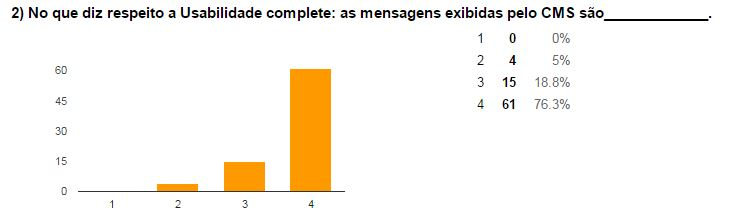
\includegraphics[keepaspectratio=true,scale=0.85]{figuras/Ques_2/q2_fig.jpg}
\caption{Frequência de respostas para a métrica de operacionalidade}
\label{res_q2-2}
\end{figure}

\begin{figure}[!htb]
\centering
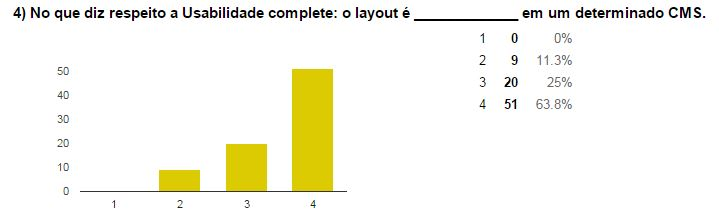
\includegraphics[keepaspectratio=true,scale=0.85]{figuras/Ques_2/q4_fig.jpg}
\caption{Frequência de respostas para a métrica de estética}
\label{res_q2-4}
\end{figure}


\begin{figure}[!htb]
\centering
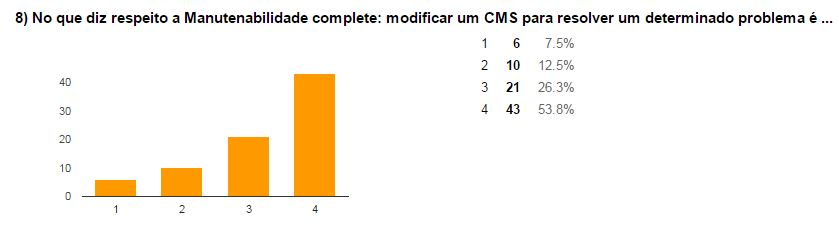
\includegraphics[keepaspectratio=true,scale=0.75]{figuras/Ques_2/q8_fig.jpg}
\caption{Frequência de respostas para a métrica de adaptabilidade}
\label{res_q2-7}
\end{figure}

\begin{figure}[!htb]
\centering
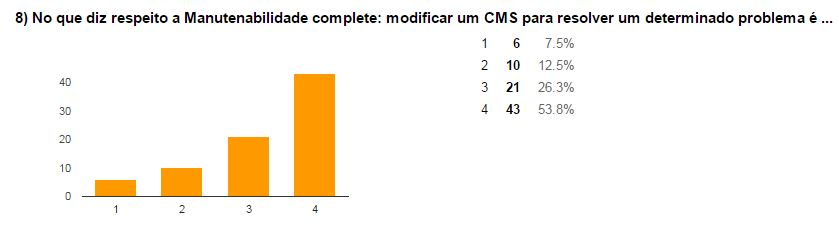
\includegraphics[keepaspectratio=true,scale=0.75]{figuras/Ques_2/q8_fig.jpg}
\caption{Frequência de respostas para a métrica de modificabilidade}
\label{res_q2-8}
\end{figure}


\begin{figure}[!htb]
\centering
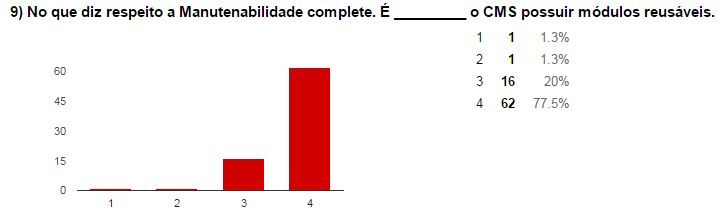
\includegraphics[keepaspectratio=true,scale=0.7]{figuras/Ques_2/q9_fig.jpg}
\caption{Frequência de respostas para a métrica de reusabilidade}
\label{res_q2-9}
\end{figure}

\clearpage

\begin{figure}[!htb]
\centering
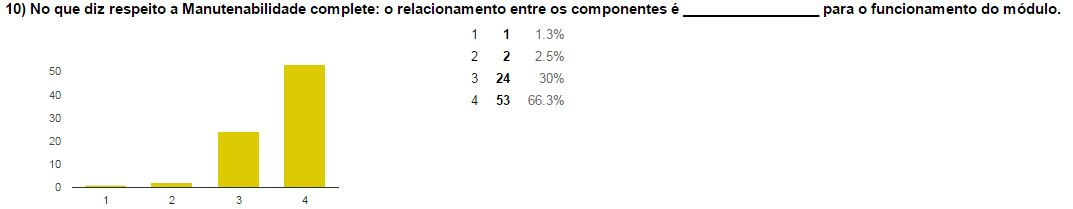
\includegraphics[keepaspectratio=true,scale=0.6]{figuras/Ques_2/q10_fig.jpg}
\caption{Frequência de respostas para a métrica de modularidade}
\label{res_q2-10}
\end{figure}

\begin{figure}[!htb]
\centering
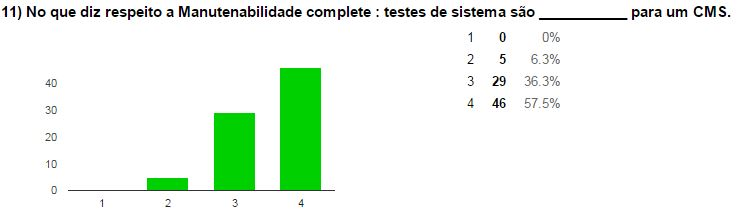
\includegraphics[keepaspectratio=true,scale=0.85]{figuras/Ques_2/q11_fig.jpg}
\caption{Frequência de respostas para a métrica de testabilidade}
\label{res_q2-11}
\end{figure}


\begin{figure}[!htb]
\centering
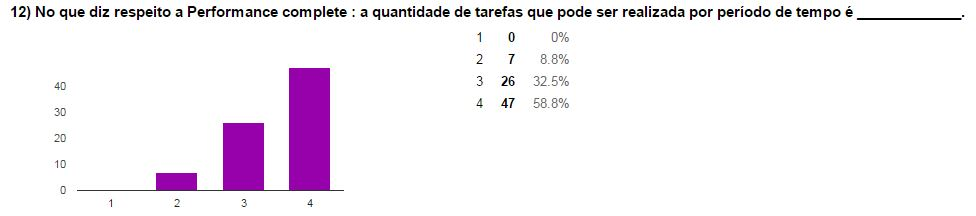
\includegraphics[keepaspectratio=true,scale=0.65]{figuras/Ques_2/q12_fig.jpg}
\caption{Frequência de respostas para a métrica de comportamento do tempo}
\label{res_q2-12}
\end{figure}

\begin{figure}[!htb]
\centering
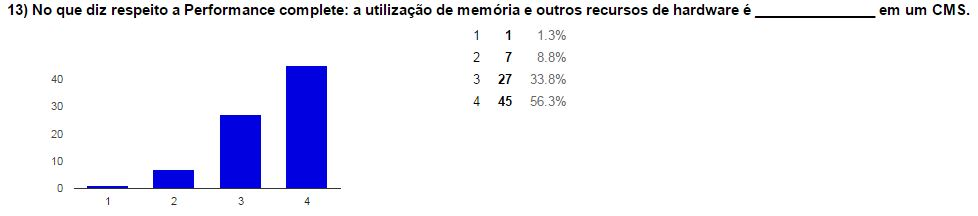
\includegraphics[keepaspectratio=true,scale=0.65]{figuras/Ques_2/q13_fig.jpg}
\caption{Frequência de respostas para a métrica de Utilização de Recursos}
\label{res_q2-13}
\end{figure}

\clearpage

\begin{figure}[!htb]
\centering
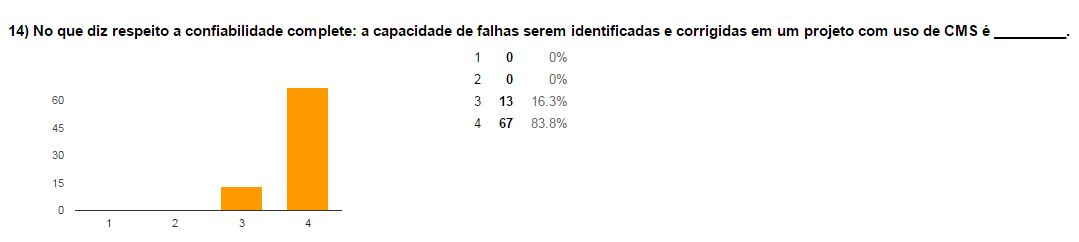
\includegraphics[keepaspectratio=true,scale=0.6]{figuras/Ques_2/q14_fig.jpg}
\caption{Frequência de respostas para a métrica de maturidade}
\label{res_q2-14}
\end{figure}

\begin{figure}[!htb]
\centering
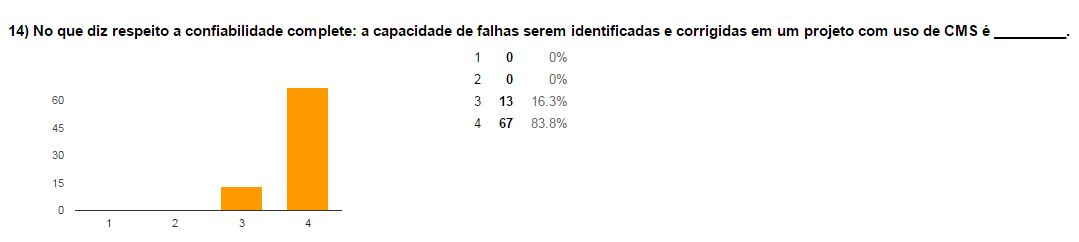
\includegraphics[keepaspectratio=true,scale=0.6]{figuras/Ques_2/q14_fig.jpg}
\caption{Frequência de respostas para a métrica de tolerância a falhas}
\label{res_q2-16}
\end{figure}


\begin{figure}[!htb]
\centering
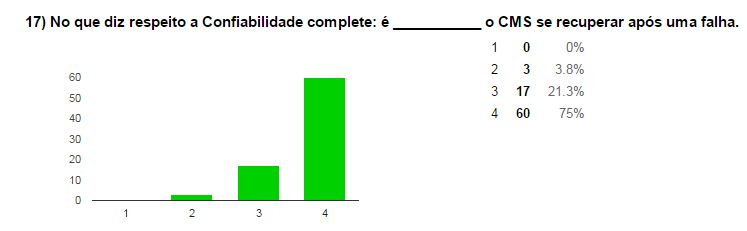
\includegraphics[keepaspectratio=true,scale=0.8]{figuras/Ques_2/q17_fig.jpg}
\caption{Frequência de respostas para a métrica de recuperabilidade}
\label{res_q2-17}
\end{figure}


\begin{figure}[!htbp]
\centering
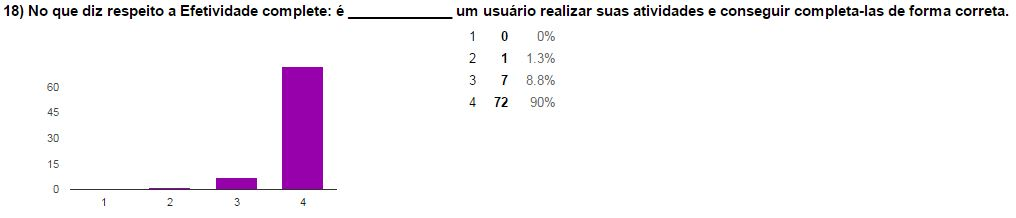
\includegraphics[keepaspectratio=true,scale=0.6]{figuras/Ques_2/q18_fig.jpg}
\caption{Frequência de respostas para a métrica de efetividade}
\label{res_q2-18}
\end{figure}
\clearpage
\begin{figure}[!htb]
\centering
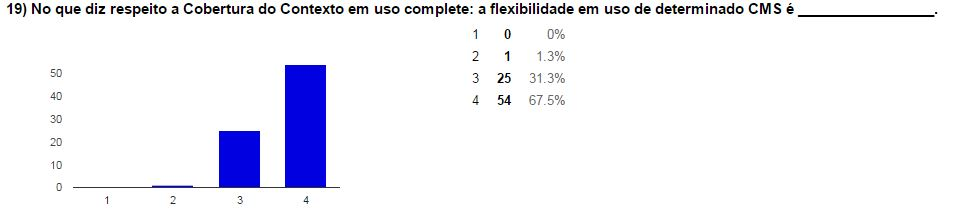
\includegraphics[keepaspectratio=true,scale=0.6]{figuras/Ques_2/q19_fig.jpg}
\caption{Frequência de respostas para a métrica de flexibilidade}
\label{res_q2-19}
\end{figure}


As Tabelas \ref{outrasmedidas1} e \ref{outras medidas 2} apresentam um resumo da média, moda, mediana e desvio padrão para as características mais importantes.

% Table generated by Excel2LaTeX from sheet 'Plan1'
\begin{table}[!htbp]
  \centering
  \caption{Outras medidas para as métricas mais relevantes}
    \begin{tabular}{llrrrrrrrr}
    \toprule
    \multicolumn{2}{l}{} & \multicolumn{1}{c}{\textbf{Q2}} & \multicolumn{1}{c}{\textbf{Q4}} & \multicolumn{1}{c}{\textbf{Q7}} & \multicolumn{1}{c}{\textbf{Q8}} & \multicolumn{1}{c}{\textbf{Q9}} & \multicolumn{1}{c}{\textbf{Q10}} & \multicolumn{1}{c}{\textbf{Q11}} & \multicolumn{1}{c}{\textbf{Q12}} \\
    \midrule
    \multicolumn{2}{l}{\textbf{Média}} & 3,7125 & 3,5250 & 3,1000 & 3,2625 & 3,7375 & 3,6125 & 3,5125 & 3,5000 \\
    \multicolumn{2}{l}{\textbf{Mediana}} & 4,0000 & 4,0000 & 3,0000 & 4,0000 & 4,0000 & 4,0000 & 4,0000 & 4,0000 \\
    \multicolumn{2}{l}{\textbf{Moda}} & 4,0000 & 4,0000 & 3,0000 & 4,0000 & 4,0000 & 4,0000 & 4,0000 & 4,0000 \\
    \multicolumn{2}{l}{\textbf{Desvio padrão}} & 0,5556 & 0,6931 & 0,8509 & 0,9513 & 0,5453 & 0,6057 & 0,6161 & 0,6560 \\
    \bottomrule
    \end{tabular}%
  \label{outrasmedidas1}%
\end{table}%

% Table generated by Excel2LaTeX from sheet 'Plan1'
\begin{table}[!ht]
  \centering
  \caption{Outras medidas para as métricas mais relevantes}
    \begin{tabular}{llrrrrrr}
    \toprule
    \multicolumn{2}{l}{} & \multicolumn{1}{c}{\textbf{Q13}} & \multicolumn{1}{c}{\textbf{Q14}} & \multicolumn{1}{c}{\textbf{Q16}} & \multicolumn{1}{c}{\textbf{Q17}} & \multicolumn{1}{c}{\textbf{Q18}} & \multicolumn{1}{c}{\textbf{Q19}} \\
    \midrule
    \multicolumn{2}{l}{\textbf{Média}} & 3,4500 & 3,8375 & 3,4125 & 3,7125 & 3,8875 & 3,6625 \\
    \multicolumn{2}{l}{\textbf{Mediana}} & 4,0000 & 4,0000 & 4,0000 & 4,0000 & 4,0000 & 4,0000 \\
    \multicolumn{2}{l}{\textbf{Moda}} & 4,0000 & 4,0000 & 4,0000 & 4,0000 & 4,0000 & 4,0000 \\
    \multicolumn{2}{l}{\textbf{Desvio padrão}} & 0,7098 & 0,3712 & 0,7745 & 0,5323 & 0,3556 & 0,5017 \\
    \bottomrule
    \end{tabular}%
  \label{outras medidas 2}%
\end{table}%

Observa-se que os desvios padrões para as questões elaboradas também são baixos, o que mostra baixa discrepância em relação a média calculada. Alguns dos fatores pelos quais podem justificar essa baixa são:

\begin{itemize}

\item Poucos sujeitos;
\item Grupo de sujeitos homogêneo, ou seja, as pessoas possuem a mesma perspectiva sobre as métricas levantadas. Fato que pode ser justificado pelo fato do questionário 2 ser um refinamento de características já mapeadas no questionário anterior.

\end{itemize}

A partir da observação dos resultados fornecidos pela análise de fatores e da estatística descritiva foi constatado que não existem métricas mais relevantes, ou menos relevantes, pois todas as métricas envolvidas possuem média alta e fazem parte de um conceito geral chamado "Qualidade de Software" de acordo com a percepção do sujeito. 

As métricas descartadas pela análise de fatores não podem ser completamente desconsideradas por terem representatividade suficiente na literatura, porém o fato de terem sido excluídas da análise de fatores aponta que tais características associadas sejam indispensáveis em um CMS, fato que pode ser experimentado por meio de trabalhos futuros com segregação e aumento no número da amostra de sujeitos.

Com as constatações feitas a partir da análise de fatores o método foi concluído. O método é bom, pois cumpre com aquilo que se propõe a fazer que é selecionar um CMS baseado em características de qualidade. Alguns refinamentos ainda podem ser feitos. Estes refinamentos estão detalhados na seção \ref{TrabalhosFuturos}.








%\subsection{Fórmula para o Número Final}
%\label{Número-Final}
%As questões definidas de acordo com o objetivo de medição foram:
%
%\begin{enumerate}
%
%\item Quanto tempo um CMS demora para realizar a uma tarefa específica?
%\citeonline{patel} em seu trabalho define como tarefas:
%\begin{itemize}
% \item A adição de texto ao CMS;
% \item A adição de plugins à página, neste caso eles consideraram um plugin de relógio e um plugin de calendário.
% \item A adição de uma imagem ao CMS.
%\end{itemize}
%
%Para o trabalho pode-se utilizar estas tarefas que \citeonline{patel} definiram em seus experimentos, assim como podem ser propostas outras tarefas além dessas.
%
%\item Quantas tarefas podem ser realizadas em um determinado CMS a cada unidade de tempo escolhida como referência ?
%%  \item Quanto de memória é utilizado para que determinado CMS possa realizar uma determinada tarefa?   
%%\textcolor{red}{Vamos repensar esta questão (Existe a possibilidade de medirmos a quantidade de memória efetivamente utilizada pelo CMS, ao invés de estimar?)}
%\item Qual o tempo de resposta do CMS quando uma determinada tarefa está sendo executada?  
%
%
%\end{enumerate}
%
%%\textcolor{red}{Poderiam ser algumas tarefas candidatas: Inserir determinado plugin. Inserir imagem. Escrever um texto. São tarefas comuns para quem usa CMS e gerencia sites.}
%
%
%\section{Métricas}
%
%A \citeonline{9126-2} apresenta algumas métricas de desempenho sob a perspectiva externa. A escolha da perspectiva externa deu-se em virtude da avaliação ter um foco de avaliação do produto já pronto e não de seu processo de desenvolvimento ou pedaços de seu proces so de desenvolvimento. 
%

%
%\begin{longtable}{|p{160pt}|p{265pt}|}
% 	\caption{Métrica Externa  - Tempo de Resposta.} \label{tipos_metricas}\\
% 	\hline
% 	 {\raggedright \textbf{Nome}}
% 	 & {\raggedright {Tempo de Resposta}}\\
% 	
% 	\hline
% 	 {\raggedright \textbf{Propósito da Métrica}}
% 	 & {\raggedright   Qual o tempo para se completar uma determinada tarefa do sistema? }\\
% 	
% 	\hline
% 	 {\raggedright \textbf{Método de Aplicação}}
% 	 & {\raggedright Iniciar uma tarefa específica.
%
%			 Medir o tempo que leva para completar a tarefa.
%
%			 Manter registro do tempo.} \\
% 	
% 	\hline
% 	 {\raggedright \textbf{Fórmula}} 
% 	 & {\raggedright  
% 	T= (Tempo em que a tarefa demorou para ser completada)
%	
%			
% 	                 } \\
%
% 	\hline
% 	 {\raggedright \textbf{Interpretação}}
% 	 & {\raggedright 0< T
%
%			 Quanto menor melhor.} \\
% 	\hline
% 	{\raggedright \textbf{Escala}}
% 	 & {\raggedright 
% 	                  Racional.
%  	                }\\
% 	
% 	\hline
% 	{\raggedright \textbf{Tipo de medição}}
% 	 & {\raggedright 
% 	                 T = Tempo de resposta.
% 	              
% }\\
% 
% 	\hline
% 	{\raggedright \textbf{Variável Independente}}
% 	 & {\raggedright T = Tempo de resposta.
% 	                  
%}\\
% 	
% 	\hline
%\end{longtable}
%
%\begin{longtable}{|p{160pt}|p{265pt}|}
% 	\caption{Métrica Externa  - Tempo Médio de Resposta.} \label{tipos_metricas}\\
% 	\hline
% 	 {\raggedright \textbf{Nome}}
% 	 & {\raggedright {Tempo Médio de Resposta}}\\
% 	
% 	\hline
% 	 {\raggedright \textbf{Propósito da Métrica}}
% 	 & {\raggedright  Qual o tempo médio de espera do usuário por uma resposta do sistema? }\\
% 	
% 	\hline
% 	 {\raggedright \textbf{Método de Aplicação}}
% 	 & {\raggedright Iniciar uma tarefa específica. Repetir várias vezes essa tarefa.
%
%			 Medir o tempo que leva para completar a tarefa.
%
%			 Manter registro dos tempos.} \\
% 	
% 	\hline
% 	 {\raggedright \textbf{Fórmula}} 
% 	 & {\raggedright  
% 	
% 	X = T(Médio)/TX (Médio).
% 	
% 	T(Médio) = $\Sigma$ Ti/N , (para i = 1 a N)
% 	
% 	TX (Médio) = Tempo de resposta necessário.
% 	
% 	Ti = Tempo de resposta para i avaliações.
% 	
% 	N = Número de avaliações realizadas.
%			
% 	                 } \\
%
% 	\hline
% 	 {\raggedright \textbf{Interpretação}}
% 	 & {\raggedright 0 <= X
%
%			 Quanto mais proximo de 1, mas não pode ser 1 .} \\
% 	\hline
% 	{\raggedright \textbf{Escala}}
% 	 & {\raggedright 
% 	                  Absoluto.
%  	                }\\
% 	
% 	\hline
% 	{\raggedright \textbf{Tipo de medição}}
% 	 & {\raggedright 
%	X = Tempo/Tempo.
% 	
% 	T(Médio) = Tempo.
% 	
% 	TX (Médio) = Tempo.
% 	
% 	Ti = Tempo.
% 	
% 	N = Contado.
% 	              
% }\\
% 
% 	\hline
% 	{\raggedright \textbf{Variável Independente}}
% 	 & {\raggedright Tempo de Resposta, Número de Avaliações Realizados
% 	                  
%}\\
% 	
% 	\hline
%\end{longtable}
%
%\begin{longtable}{|p{160pt}|p{265pt}|}
% 	\caption{Métrica Externa - Tempo de Rendimento} \label{tipos_metricas}\\
% 	\hline
% 	 {\raggedright \textbf{Nome}}
% 	 & {\raggedright {Tempo de Rendimento}}\\
% 	
% 	\hline
% 	 {\raggedright \textbf{Propósito da Métrica}}
% 	 & {\raggedright  Quantas tarefas podem ser realizadas com sucesso em um determinado período de tempo? }\\
% 	
% 	\hline
% 	 {\raggedright \textbf{Método de Aplicação}}
% 	 & {\raggedright 
% 	 
% 	 Estabelecer um período de tempo aceitável.
% 	 
% 	 Iniciar várias tarefas específicas ao mesmo tempo. .
%
%	 Medir o tempo que leva para completar a tarefa.
%
%	Manter registro dos tempos.} \\
% 	
% 	\hline
% 	 {\raggedright \textbf{Fórmula}} 
% 	 & {\raggedright  
% 	
% 	X = A/T.
% 	
% 	A = Número de tarefas completadas.
% 	
% 	T = Período de tempo observado.
%			
% 	                 } \\
%
% 	\hline
% 	 {\raggedright \textbf{Interpretação}}
% 	 & {\raggedright 0 < X
%
%			 Quanto maior melhor .} \\
% 	\hline
% 	{\raggedright \textbf{Escala}}
% 	 & {\raggedright 
% 	                  Racional.
%  	                }\\
% 	
% 	\hline
% 	{\raggedright \textbf{Tipo de medição}}
% 	 & {\raggedright 
%	A = Contado.
%	
%	T = Tempo.
%	
%	X = Contado/Tempo.
% 	              
% }\\
% 
% 	\hline
% 	{\raggedright \textbf{Variável Independente}}
% 	 & {\raggedright Número de tarefas completadas, Período de tempo observado.
% 	                  
%}\\
% 	
% 	\hline
%\end{longtable}
%
%% \begin{longtable}{|p{160pt}|p{265pt}|}
%%  	\caption{Métrica Externa - Proporção de erros de memória / tempo} \label{tipos_metricas}\\
%%  	\hline
%%  	 {\raggedright \textbf{Nome}}
%%  	 & {\raggedright {Proporção de erros de memória / tempo}}\\
%%  	
%%  	\hline
%%  	 {\raggedright \textbf{Propósito da Métrica}}
%%  	 & {\raggedright  Quantos erros de memória foram encontrados ao longo de um determinado período de tempo especificado de utilização de recursos? }\\
%%  	
%%  	\hline
%%  	 {\raggedright \textbf{Método de Aplicação}}
%%  	 & {\raggedright 
%%  	 Estabelecer umperíodo de tempo para a simulação.
%% 
%%  	 
%% 	 Simular uma condição
%% 	 em que o sistema atinja uma situação de carga máxima.
%% 
%% 	 
%% 	 Executar a aplicação e registrar a quantidade de falhas de memória.
%% 	 
%% 	  	 
%%  	 } \\
%%  	
%%  	\hline
%%  	 {\raggedright \textbf{Fórmula}} 
%%  	 & {\raggedright  
%%  	X = A/T.
%%  	
%%  	A = Número de mensagens de alerta ou falhas de sistema
%%  	
%%  	T = Tempo de observação.
%% 			
%%  	                 } \\
%% 
%%  	\hline
%%  	 {\raggedright \textbf{Interpretação}}
%%  	 & {\raggedright 
%% 			 0 < = X.
%% 			 
%% 			 Quanto menor melhor .} \\
%%  	\hline
%%  	{\raggedright \textbf{Escala}}
%%  	 & {\raggedright 
%%  	                  Racional.
%%   	                }\\
%%  	
%%  	\hline
%%  	{\raggedright \textbf{Tipo de medição}}
%%  	 & {\raggedright 
%% 	A= Contado.
%% 	
%% 	T = Tempo.
%% 	
%% 	X = Contado/Tempo.
%%  	              
%%  }\\
%%  
%%  	\hline
%%  	{\raggedright \textbf{Variável Independente}}
%%  	 & {\raggedright A = Número de mensagens de alerta ou falhas de sistema
%%  	
%%  	T = Tempo de observação.
%%  	                  
%% }\\
%% 	
%%  	\hline
%% \end{longtable}
%
%
%\subsection{ Sumário de métricas }
%
%Com o objetivo de mapear as questões e métricas encontradas com realização do GQM. A imagem \ref{sum_metricas} tem o objetivo de fornecer um modelo para a organização das medições que serão realizadas no TCC 2.
%
%\begin{figure}[htpb!]
%\centering
%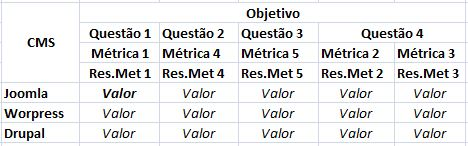
\includegraphics[keepaspectratio=true,scale = 1.0]{figuras/sum_metricas.JPG}
%\caption{Sumário de Métricas.}
%\label{sum_metricas}
%\end{figure}
%
%
%
%% \begin{table}[!htpb]
%% \caption{Cronograma das atividades previstas}
%% \label{t_cronograma}
%% \centering
%% 
%% % definindo o tamanho da fonte para small
%% % outros possíveis tamanhos: footnotesize, scriptsize
%% \begin{small} 
%%   
%% % redefinindo o espaçamento das colunas
%% \setlength{\tabcolsep}{3pt} 
%% 
%% % \cline é semelhante ao \hline, porém é possível indicar as colunas que terão essa a linha horizontal
%% % \multicolumn{10}{c|}{Meses} indica que dez colunas serão mescladas e a palavra Meses estará centralizada dentro delas.
%% 
%% \begin{tabular}{|c|c|c|c|c|c|c|c|c|c|c|c|c|c|c|c|c|c|c|c|c|c|c|c|c|}\hline
%%  & \multicolumn{24}{c|}{Objetivo}\\ \cline{2-25}
%%  \multicolumn{5}{|c|}{Questões}\\ \cline{2-25}
%% \raisebox{1.5ex}{CMS} & 01 & 02 & 03 & 04 & 05 & 06 & 07 & 08 & 09 & 10 & 11 & 12 & 13 & 14 & 15 & 16 & 17 & 18 & 19 & 20 & 21 & 22 & 23 & 24 \\ \hline
%% 
%% Joomla & X & X & X & X & X & X & X & X & X & X & X & X & & & & & & & & & & & & \\ \hline
%% WordPress & & X & X & X & X & X & X & X & X & X & X & X & & & & & & & & & & & & \\ \hline
%% Drupal & & X & X & X & X & X & X & X & X & X & X & X & X & X & X & X & X & X & X & X & & & & \\ \hline
%% 4 & & X & X & X & X & X & X & X & X & X & X & X & X & X & X & X & X & X & X & X & & & & \\ \hline
%% 5 & & X & X & X & X & X & X & X & X & X & X & X & X & X & X & X & & & & & & & & \\ \hline
%% 6 & & X & X & X & X & X & X & X & X & X & X & X & X & X & X & X & X & X & X & X & X & & & \\ \hline
%% 7 & & & & X & X & X & X & X & X & X & X & X & X & X & X & X & X & X & X & X & X & X & & \\ \hline
%% 8 & & & & & & X & X & X & X & X & X & X & X & X & X & X & X & X & X & X & X & X & X & X \\ \hline
%% 
%% \end{tabular} 
%% \end{small}
%% 
%% \end{table} 
%% 
%
\chapter[Conclusões]{Conclusões}
\label{final}


O uso de CMS para o desenvolvimento de páginas web permite ao desenvolvedor publicar e editar conteúdos sem um conhecimento pleno de linguagens de programação para web. Além disso, o desenvolvedor possui a liberdade de adicionar novas funcionalidades, ou mudar o design da sua página por meio do uso de plugins e templates. 

Por serem boas alternativas para o desenvolvimento web, a quantidade de CMSs disponíveis no mercado é bastante significativa. Devido ao grande número de CMSs disponíveis, escolher a melhor opção para um determinado contexto pode não ser algo simples. Contextos que podem variar desde aplicações para e-commerce, redes sociais, revistas eletrônicas, blogs, sites para instituições bancárias e outros, são contextos usados com frequência por quem utiliza CMS. 

Em outras palavras, a escolha de um CMS pode influenciar várias caractecterísticas funcionais, ou não funcionais de uma determinada aplicação web. A partir desta motivação, o estudo de critérios que facilitem a escolha de produtos do tipo CMS foi importante para esta pesquisa. 

Motivação que serviu como base para a seguinte questão de pesquisa: 

"\textbf{{Como estabelecer um método objetivo para a escolha de CMSs a serem utilizados no desenvolvimento de sites Web?}}"
  
Questão de pesquisa que fundamentou-se no seguinte objetivo geral:

"\textbf{Propor um método objetivo que possa servir de apoio para a escolha de um CMS.}"

Para atender ao objetivo geral foram definidos seis objetivos específicos, que foram resolvidos ao longo do trabalho de conclusão de curso.

Para o objetivo específico número um \textit{"Identificar o que é um CMS"} foi realizado um estudo a respeito do que é CMS, quais as vantagens e desvantagens do uso de CMS para o desenvolvimento web, algumas aplicações feitas com auxílio de CMSs. Após esse estudo foi definido dois critérios importantes para o estudo: o licenciamento, que compreende o fato de um CMS ser software livre ou proprietário e a popularidade. Essas definições de estudo estão presentes no Capítulo \ref{CMS} deste trabalho.

Para o objetivo específico dois
\textit{"Examinar conceitos de qualidade de software, a fim de esclarecer como medir as características de sistemas CMSs, a fim de permitir que elas sejam mensuradas"} foi realizado um estudo a respeito da ISO/IEC 25000, série SQuaRE de normas. Neste estudo foi abordado a sua organização, a sua visão de qualidade em uso e qualidade do produto e um comparativo com a antiga ISO/IEC 9126. Essas definições de estudo estão presentes no Capítulo \ref{Qualidade_de_Software} deste trabalho.

Para o objetivo específico três 
\textit{"Definir medições para avaliar as características de CMSs a partir de conceitos das teorias para estabelecer medições usadas na Engenharia de Software"} foi realizado um estudo sobre tipos de métricas de software, sobre escalas de software e sobre métodos para a elaboração de métricas de software. Métodos que compreendem o \textit{Goal, Question, Metric}-GQM e o \textit{Pratical Software Measurement}-PSM. Este estudo foi abordado no Capítulo \ref{metrics}.

Para o objetivo específico quatro
\textit{"Identificar sistemas de CMSs candidatos para serem usados como estudos de caso na aplicação do método proposto"} foi realizado um estudo a respeito do licenciamento e da popularidade em sistemas CMS. Durante esse estudo foram citados diversos CMSs, porém com a a aplicação dos critérios de software livre, popularidade e tamanho de comunidade. O tamanho da comunidade foi medido por meio de redes sociais e o número de commits no github. A partir dos filtros aplicados o número de CMSs se reduziu aos mais populares: Joomla, Wordpress e Drupal. Este estudo foi abordado na Seção \ref{CMSs_candidatos} do Capítulo \ref{CMS}. 

Para o objetivo específico cinco
" Estabelecer um método que possa ser aplicado aos CMSs candidatos, a partir de medições oriundas de conceitos de qualidade de software" foi realizado um levantamento de características de CMS com base na literatura. As características citadas na literatura foram mapeadas com suas respectivas características SQuaRE. Este mapeamento teve como objetivo agrupar as características  semelhantes e mais citadas para a elaboração de um \textit{survey}. \textit{Survey} que foi submetido e respondido por especialistas para elencar as características de CMS mais relevantes.

Após o estudo do survey as características mais relevantes foram  agrupadas em dois grupos. O grupo um foi composto por características que não podem ser mensuradas pela Square, já o dois pelas que podem. A partir disso, foi definida uma visão geral para o método (Seção \ref{Visao_Método}) que foi dividido em duas partes quanto a sua execução. Para a 2ª parte do método foi feito um GQM com a finalidade de definir as métricas necessárias para o estudo. Estas definições de estudo foram apresentadas no Capítulo \ref{aplicação}.

Para o último objetivo específico \textit{"Validar o método proposto a partir de opiniões de especialistas no assunto "} foi feito um segundo survey com o objetivo de validar as métricas elaboradas para o método proposto. Os resultados para este \textit{survey} foram citados na Seção \ref{resultados_quest2}. Para a validação do \textit{survey} foi aplicado o método da análise de fatores. Para prosseguir com o método da análise  de fatores foi necessário produzir uma matriz de dados e verificar a validade da mesma. Para aferir a validade foram utilizados três indicadores. Esses indicadores foram: o $\alpha$ de Cronbach, o KMO e o BTS. 

Depois da validação da matriz de dados elaborada constatou-se que a mesma podia ser quebrada em fatores. A partir da validação foi iniciada a extração de fatores com rotação da matriz. Foi gerado um gráfico de declividade, no qual foram sugeridos seis fatores. Inicialmente os seis fatores foram observados, porém verificou-se a necessidade da redução em menos fatores, pois os conceitos associados aos fatores não eram compatíveis com a literatura.

As reduções foram feitas até se chegar a um único fator. Este fator foi nomeado de métricas mais significativas. Porém, foi constatado que conceitos importantes para a literatura não foram considerados pela análise de fatores. Estes conceitos foram a Segurança e a Adequação Funcional.    

A causa para a desconsideração desses conceitos deve ser atribuída ao baixo número de sujeitos. Foram 80 sujeitos para 19 questões mapeadas, o que leva a uma média de 4 sujeitos por item.  

A partir do método da análise de fatores foi percebido que um passo critico para o método proposto é a escolha de características a partir dos critérios
que dizem respeito ao tipo de site que será produzido, uma vez que, as métricas selecionadas representam o conceito geral de Qualidade de Software para a opinião dos sujeitos entrevistados. Os critérios apresentados para a escolha de CMSs de acordo com a aplicação a ser desenvolvida estão na Seção \ref{passo_parteII_metodo} deste trabalho.   


Após a avaliação do método por especialistas concluiu-se o método. A grande contribuição do método para a indústria de software foi que com a sua utilização é possível o desenvolvedor testar se o CMS é adequado a uma determinada característica. Característica que caso venha a ser importante para uma determinada aplicação pode ser avaliada por meio de métricas estabelecidas no método, e então, avaliar se o CMS é adequado para a aplicação em questão. 

%Após o trabalho realizado o método foi proposto atendendo aos objetivos geral e específicos.   

\section{Sugestões de Trabalhos Futuros}
\label{TrabalhosFuturos}

Apesar do método estar de acordo com a visão dos especialistas, conforme foi mostrado nos questionários aplicados. A visão dos especialistas encontrados reflete apenas a visão de quem usa, ou usou um CMS software livre para os seus projetos. A visão de especialistas ligados ao uso de CMSs proprietários poderia também ser abordada. Para isso poderiam ser realizadas entrevistas com desenvolvedores que trabalham com CMSs proprietários em um determinado ambiente organizacional, afim de colher opniões e obter uma amostra mais refinada de características para refinar o método proposto.

Uma validação por experimentos também poderia ser executada. Para esta validação poderia ser escolhido um número "X" de CMSs, e em seguida os CMSs escolhidos seriam submetidos aos passos descritos nas Seções \ref{M_ParteI} e \ref{M-Parte-II}. Durante o experimento o foco poderia ser a análise de uma característica como por exemplo, a Usabilidade. A partir da aplicação deste experimento poderia ser verificado se os CMSs "X" escolhidos atenderiam a característica de Usabilidade por meio das métricas propostas.

As metas para as medições propostas são apenas sugestões. Estas metas poderiam ser verificadas propondo-se vários experimentos quantitativos com a aplicação das próprias métricas sugeridas envolvendo um conjunto de CMSs escolhidos.

Devido ao baixo número de sujeitos (4/item) a reaplicação do método de análise de fatores deve ser considerada. Um bom número de sujeitos seria (10/item), o que equivaleria a 190 sujeitos. A partir disso, também seria necessária uma reaplicação do questionário de validação de métricas, considerando uma validação semântica do questionário a fim de melhorar o instrumento de coleta e possibilitar melhores resultados. 

Apesar de conceitos importantes terem sido desconsiderados, no resultado final da análise de fatores, as métricas mais significativas representam o conceito geral de qualidade de software para a opnião dos especialistas entrevistados. 
Opniões que poderiam ser agrupadas quanto a experiência (desenvolvedor, usuário, mantenedor) do especialista em relação ao uso de CMS. Possibilitando uma nova sugestão para reaplicação do método de análise de fatores, a fim de perceber se a acurácia dos fatores seria melhorada. 

Além disso, uma investigação mais profunda dos conceitos indispensáveis para sistemas CMSs se faz necessária devido aos resultados encontrados com a análise de fatores.  
%Este capítulo apresenta as considerações finais, acerca do trabalho desenvolvido e as sugestões de trabalhos futuros que podem ser derivados desta pesquisa.

%\section{Considerações Finais} 


%
%Após a execução deste trabalho cumpriu-se com o 1ª objetivo específico no capítulo \ref{CMS} onde foram apresentadas a definição do que é um CMS, suas vantangens e desvantagens,  seus objetivos e os critérios de escolha para os CMSs que serão alvo de estudo no TCC2. Esses critérios foram a forma de distribuição do software: Software Livre ou Software proprietário e a popularidade. Além disso, foi explicada a importância de requisitos não funcionais, destacando os requisitos não funcionais de desempenho, o principal alvo de estudo deste TCC.
%
%Para o objetivo específico 2 este trabalho apresentou conceitos da importância da qualidade de software no processo de desenvolvimento. Apresentou conceitos chaves de qualidade de software, tais como qualidade interna, qualidade externa e qualidade em uso, além de destacar a importância da \citeonline{9126} no contexto de qualidade de software. Além de uma definição sobre o que são métricas, seus tipos e escalas. E por fim o capítulo apresentou como o PSM e o GQM ajudam a projetar métricas para a aferir a qualidade de software.
%
%Para o objetivo específico 3 este trabalho o capítulo \ref{aplicação} utilizou os conceitos do GQM para a montagem do framework de métricas baseado também na \citeonline{9126}.
%
%Este trabalho definiu uma investigação consistente para que no TCC 2 as métricas possam ser aplicadas nos CMSs escolhidos a fim de dar um melhor suporte para quem quer um melhor desempenho de seus websites e deseja usar uma solução envolvendo CMS.
%
%Assim sendo, considerando o cumprimento dos objetivos específicos, foi considerado como cumprido o objetivo geral da pesquisa deste TCC, ou seja: \textit{"Estudar CMS de forma a identificar  características de desempenho que possam ser usadas  na definição de critérios de escolha de um determinado CMS
%a serem usados no desenvolvimento de um sistema padrão WEB".}
%
%\section{Considerações Finais}
%
%Levando em consideração as características abordadas neste trabalho. Os mesmos princípios que foram usados para elaborar métricas de desempenho podem ser usados para a elaboração de outras métricas que avaliem outras características não funcionais, tais como usabilidade, manutenibilidade, confiabilidade dentre outras características. Além de também poder levar em consideração a perspectiva interna das métricas de desempenho. Essas observações levariam a diversos trabalhos futuros com objetivos semelhantes.
%
%Para o TCC 2 pretende-se submeter as métricas escolhidas à avaliação de um especialista, para que o mesmo possa julgar se tais métricas são aplicáveis dentro de um contexto de um CMS específico e então atuar como um filtro para que seja considerado apenas o necessário. O especialista também poderá acrescentar métricas que conheça e que possam contribuir para a evolução do trabalho. Após a consolidação das métricas será feita uma pesquisa sobre quais ferramentas podem ser usadas para levantar os dados das métricas, depois um ambiente de execução terá que ser elaborado por fim haverá a coleta de dados e as conclusões finais deste trabalho.  